%\documentclass{acm_proc_article-sp}
\documentclass{sig-alternate}
%\documentclass{vldb}

%%
%% include packages
%%
\usepackage{times}                    %% for time fonts if needed
\usepackage{amsmath}                  %% for math
\usepackage{tabularx}                 %% resize tables
\usepackage{colortbl}                 %% put some color to tables
\usepackage{multirow}                 %% multi-rows/columns on tables
\usepackage{booktabs}                 %% more for tables
\usepackage{tikz}                     %% tikz drawing package
\usepackage{graphicx}                 %% include graphics
\usepackage{algorithm}                %% algorithm floated enviroment
\usepackage{algorithmic}              %% algorithm enviroment
\usepackage{balance}

%%
%% (re)new
%%
\newtheorem{theorem}{Theorem}
\newtheorem{lemma}[theorem]{Lemma}
\newtheorem{definition}{Definition}

%%macros
\newcommand{\la}{\langle}
\newcommand{\ra}{\rangle}
\newcommand{\smp}{\mathcal{S}}
\newcommand{\prob}{\mathcal{P}}
\renewcommand{\tt}{\texttt}
\renewcommand{\rm}{\textrm}
\renewcommand{\sf}{\textsf}
\renewcommand{\it}{\textit}
\renewcommand{\bf}{\textbf}
\newcommand{\md}{\textmd}
\renewcommand{\sc}{\textsc}


\begin{document}
\conferenceinfo{SIGMOD'13,} {June 22--27, 2013, New York, New York, USA.}
\CopyrightYear{2013}
\crdata{978-1-4503-2037-5/13/06}
\clubpenalty=10000
\widowpenalty = 10000

\title{Column Imprints: A Secondary Index Structure}
\numberofauthors{2}
\author{
\alignauthor Lefteris Sidirourgos\\
\affaddr{CWI}\\
\affaddr{Amsterdam, The Netherlands}\\
\email{lsidir@cwi.nl}
\alignauthor Martin Kersten\\
\affaddr{CWI}\\
\affaddr{Amsterdam, The Netherlands}\\
\email{mk@cwi.nl}
}

\maketitle

\begin{abstract}
Large scale data warehouses rely heavily on secondary indexes, such as bitmaps
and b-trees, to limit access to slow IO devices. However, with the advent
of large main memory systems, cache conscious secondary indexes are needed to
improve also the transfer bandwidth between memory and cpu. In this paper, we
introduce \it{column imprint}, a simple but efficient cache conscious secondary
index. A column imprint is a collection of many small bit vectors, each
indexing the data points of a single cacheline. An imprint is used during query
evaluation to limit data access and thus minimize memory traffic. The
compression for imprints is cpu friendly and exploits the empirical observation
that data often exhibits local clustering or partial ordering as a side-effect
of the construction process. Most importantly, column imprint compression
remains effective and robust even in the case of unclustered data, while other
state-of-the-art solutions fail. We conducted an extensive experimental
evaluation to assess the applicability and the performance impact of the column
imprints. The storage overhead, when experimenting with real world datasets, is
just a few percent over the size of the columns being indexed. The evaluation
time for over 40000 range queries of varying selectivity revealed the
efficiency of the proposed index compared to zonemaps and bitmaps with WAH
compression.
\end{abstract}

% A category with the (minimum) three required fields
\category{H.3}{Information Storage and Retrieval}{Content Analysis and Indexing}
%\category{H.3}{Information Systems Applications}{Miscellaneous}
%A category including the fourth, optional field follows...
%\category{D.2.8}{Software Engineering}{Metrics}[complexity measures, performance measures]
%\terms{Theory}
\keywords{Secondary Index; Columnar Databases;} % NOT required for Proceedings

\section{Introduction}\label{sec:intro}

Indexes are a vital component of a database system. They allow the system
to efficiently locate and retrieve data that is relevant to the users' queries. Despite the large body of research literature, just a few solutions have found
their respective places in a database system~\cite{BKS+90,HNP95,IKM07,OQ97}.
Nevertheless, the pursuit for more efficient and succinct indexing structures
remains.

Indexes are divided into \it{primary} and \it{secondary} according to their
ability to govern the placement of the data. Primary indexes combine
navigational structures with physical data clustering to achieve fast access.
The benefit is that relevant data is placed in adjacent pages and thus
significantly improving the evaluation of range queries. However, each
additional primary index on the same relation calls for a complete copy of the
data, rendering the storage overhead prohibitive. Similarly, secondary indexes
are auxiliary structures that speed up search, but they do not change the order
of the data in the underlying physical storage. Secondary indexes are typically
much smaller than the referenced data and, therefore, faster to access and
query. However, retrieving the relevant data from disk can be a costly
operation since it may be scattered over many pages. As long as the time to
scan the secondary index is significantly less than accessing the data, and the
selectivity of the query is high, secondary indexes can significantly improve
the query evaluation time.

Most structures designed for primary indexing, such as B-tree and hash tables,
can also be used for secondary indexing. However, they are not as lightweight
as one would wish. Bitmaps, or variations of bitmaps, are more often used for
this task~\cite{WLO+85}. Bitmaps work by mapping individual values to an array
of bits. At query time, the bitmap is examined and whenever the bits that
correspond to the query's predicates are set, the mapped data is retrieved for
further processing. Bitmaps are traditionally used for attributes with low
cardinality~\cite{ON87}, although bit-binning techniques make them suitable
for larger domains too~\cite{CI99,SW07}.

With the introduction of column stores and the shift of the memory
bottleneck~\cite{MKB09}, the need for designing \it{hardware-conscious}
secondary indexes becomes more evident. In a main memory DBMS, the problem
of efficiently accessing disk blocks is replaced with the problem of
minimizing cache misses. In addition, algorithms require a more
careful implementation. There is much less design space to hide an inefficient
implementation behind the latency of accessing a disk block.

A second paradigm shift concerns the volume and the nature of the data. Most
notable of them all are scientific database applications that stress the limits
of modern designs by including hundreds of attributes in a single relation. In
addition, the value domains are often of double precision, rather than the
traditional categorical ones encountered in business applications.
Column stores are the prime candidates for providing solutions for such
demanding applications. On high-end servers, with large main memories, it is
even possible to keep many columns with billions of elements in memory over a
long period of time. Nevertheless, fast access, supported by light-weight
indexing structures, remains in demand to improve the interactive scientific
exploration process.

To address these challenges, we propose a simple but efficient secondary
indexing structure, called \it{column imprints}. A column imprint is a cache
conscious secondary indexing structure suitable for both low and high
cardinality columns. Given a column with values from domain $\mathcal{D}$, we
derive a small sample to approximate a histogram of a few (typically 64 or
less) equal-height bins. The entire column is then scanned, and for every
cacheline of data, a bit vector is created. The bits in each vector correspond
to the bins of the histogram. A bit is set if at least one value in the
cacheline falls into the corresponding bin. The resulting bit vector is an
\it{imprint} of the current cacheline that describes which buckets of the
approximated histogram the values of the cacheline fall into. The collection of
all the resulting bit vectors form a unique \it{column imprint}. Consequently,
by examining an imprint of a column, the execution engine can decide --in
a cacheline granularity-- which parts of the column data are relevant to the
query predicates, and only then fetch them for further processing. A column
imprint is particularly suited for evaluating both range and point queries on
unsorted data. Contrary to existing work, a column imprint is a \it{non-dense}
bit indexing scheme, i.e., only one bit is set for all equal values in a
cacheline, instead of the traditional approach where each data point is always
mapped to a different bit.

To reduce the memory footprint of a column imprint, we introduce a simple
compression scheme based on a run-length encoding of imprints. Consecutive and
identical bit vectors are compressed together and annotated with a counter.
Paraphrasing, our compression
schema can be characterized as row-wise, i.e., it compresses bit vectors
horizontally, contrary to the more common column-wise approach that partitions
a bitmap vertically and compress it per column~\cite{WOS02}. The horizontal
compression exploits our empirical observation that, in most data warehouses
that we explored, data suitable for secondary indexing exhibits, in the
cacheline level, some degree of clustering or partial ordering. These desirable
properties stem either from the regular and canonical data insertion procedure,
or from the production of the data itself, or even indirectly imposed by the
other primary indexed attributes of the same relation. Column imprints are
designed such that any clustering or partial ordering is naturally exploited
without the need for extra pasteurization. In other words, they are less
susceptible to the order in which individual values appear in a cacheline,
while more opportunities for compression are presented. In addition,
because of this immunity to value order within a cacheline, a column imprint
remains robust even in the case of highly unclustered data. We experimentally
demonstrate that imprints perform well and behave as intended even in the
presence of skewed data, where other state-of-the-art bitmap compression
techniques, such as WAH~\cite{WOS02}, are less effective.

The contributions of our work can be summarized as follows:
\begin{itemize}
\item We introduce column imprints, a light-weight secondary index
structure for main memory database systems.
\item We detail the algorithms and the implementation details for constructing
and compressing a column imprint.
\item We present the algorithms to efficiently evaluate range queries with the
use of column imprints.
\item We study the effect on imprints when updating the values of a column.
\item We quantify the amount of local clustering by introducing
a metric called \it{column entropy}.
\item We conduct an extensive comparative experimental evaluation of
the imprint index structure using thousands of columns taken from several
real-world datasets.
\end{itemize}

The remainder of the paper is organized as follows. In
Section~\ref{sec:construction} we detail the ideas and the algorithms for
constructing a column imprint. In Section~\ref{sec:operators} we present the
algorithms for querying the proposed index. Next, we study the different cases
of updating column imprints in Section~\ref{sec:updates}.
Section~\ref{sec:background} presents the related work. In
Section~\ref{sec:evaluation} we present an extensive experimental evaluation
for column imprints. We conclude in Section~\ref{sec:conclusions}.

\section{Secondary Index with Imprints}\label{sec:construction}

An imprint index is an efficient and concise secondary index for range and
point queries. It is designed for columnar databases where multiple
memory-resident or memory-mapped columns are repeatedly scanned.
Imprints provide a coarse-grain filtering over the data, aimed at
reducing expensive loading from memory to the cpu cache. Deployment of column
imprints is suited for those cases where alternative properties do not hold.
For example, if a column is already sorted, the proper use of binary search
algorithms largely alleviates the overhead of accessing non-relevant memory
pages. If the data is appended out of order, or the order is disturbed by
updates, then column imprints can be considered as a fast access method to
locate relevant data. An efficient column imprint maximizes the filtering
capabilities with minimal storage overhead.

Columnar databases decompose a relation into its attributes and sequentially
store the values of each column. This differs from the traditional approach of
row-stores that place complete tuples in adjacent pages. To enable tuple
reconstruction in a column store, an ordered list of \it{(id, value)} pairs is
maintained, where \it{id}s are unique and increasing identifiers. Values from
different columns, but with the same \it{id}, belong to the same tuple.
Typically, a column is implemented by a single dense array, thus \it{id}s need
not be materialized since they can be easily derived from the position of the
values in the array.
%
%\begin{figure}
%\centering\includegraphics{figs/example3.eps}
%\caption{A simple column and an example of zonemaps, bitmaps, and \it{imprints} indexes.}
%\label{fig:example}
%\end{figure}

Figure~\ref{fig:example} shows a column with 15 integer values in the range
of 1 to 8. The values are unsorted because the column corresponds to one of the
unordered attributes of a relation. In the absence of any secondary index, a
complete scan is needed to locate all values that satisfy the predicates of a
query. The result of such a scan is the positions in the array of the qualifying
values. It is preferred to return the positions rather than the actual values
because of the \it{late materialization} strategies usually used in column
stores~\cite{AMD+07}. However, instead of scanning the entire column, secondary
indexes can be used to avoid accessing data that is certain not to be part
of the query result.

\subsection{State of the Art in Secondary Indexes}

Zonemaps is a common choice for indexing secondary attributes. A zonemap index
notes the minimum and the maximum values found across a predefined number of
consecutive values, called the zones. The zonemap index of
Figure~\ref{fig:example} partitions the column into $5$ zones. In this example,
each zone has the size of a cacheline that fits exactly $3$ values. The first
zone contains the values $1$, $8$, and $4$. The minimum value is $1$ and the
maximum is $8$. Similarly, for the second zone the minimum value is $1$ and
maximum $6$, and so on for the remaining zones. To evaluate a query using
zonemaps, the minimum and maximum values of each zone are compared with the
predicates of the query. If the predicates' ranges overlap with the range of
a zone, then the zone (i.e., the cacheline) is retrieved and the
exact positions of only the \it{qualifying} values are returned. Note that the
ranges of the predicates and the zone may overlap but not be strictly
inclusive.

\begin{figure}
\centering\includegraphics{figs/example3.eps}
\caption{A simple column and an example of zonemaps, bitmaps, and \it{imprints} indexes.}
\label{fig:example}
\end{figure}

Bitmaps are another popular choice for secondary indexing. They work by
mapping the column domain to bit vectors. Each vector has as many bits as the
size of the column. For each value found in a specific position of the column,
the corresponding bit in the mapping bitvector is set. The mapping can be $1-1$
if the cardinality of the column is low, or $N-1$, with the help of binning
strategies, if the cardinality is high. A bitmap index uses significantly less
storage than the column, thus making it cheaper to scan. Deciding if a value
satisfies a query involves first checking the corresponding
bitmap, and returning only the position of the bits that are set. The checking
is done with bitwise operators, making the process faster than the value
comparison needed by zonemaps. Figure~\ref{fig:example} details a bitmap index
with 15 bits per bit vector, where each bit corresponds to one position of the
column. There are 8 such bit vectors (drawn vertically in the figure), where
the first one maps value $1$, the second one value $2$, and so on. Bits
are set as follows: the $11$th position of the column contains the value $5$,
therefore, in the $5$th bit vector, the $11$th bit is set. Similarly, the
$3$rd value of the column is $4$, hence the $3$rd bit of the $4$th bitmap is
set. In this example there is a 1-1 mapping between the eight unique values of
the column and the eight vectors of the bitmap index.

\subsection{Column Imprints}

We propose \it{column imprints} as an alternative secondary index that best
combines the benefits of the aforementioned state-of-the-art indexes.
Column imprints map the values of a column to a vector of bits. However,
instead of allocating one such vector per value, imprints allocate one
vector per cacheline. We call the vectors of a column imprints index
\it{imprint vectors} to distinguish them from the bitvectors of a bitmap
index. An imprint vector does not have only one bit set per position, but as
many bits as are needed to map all distinct values of a cacheline. To decide if
a cacheline contains values that satisfy the predicates of a query, first
the imprint vectors are checked. If at least one common bit between the
bitvector that maps the query's predicates and the imprint vector is set, then
the entire cacheline is fetched for further processing. The imprint is checked
with the bitwise operator \tt{AND} thus making the initial filtering very fast,
while the number of imprint vectors to be checked is significantly reduced
because of having one per cacheline instead of one per value. The rightmost
index in Figure~\ref{fig:example} depicts the imprint index of the example
column. Each imprint vector uses 8 bits per cacheline, while three
bits are set. The partitioning of the column is done per
cacheline, same as the zones of the zonemap index. The imprint vector
corresponding to the first cacheline has the $1$st, $4$th, and $8$th bit
set, since the first three values of the column are $1$, $8$ and $4$. For the
second cacheline the $1$st, $6$th, and $7$th bits are set, and so on
for the rest of the cachelines. There are in total five imprint
vectors to index the column of Figure~\ref{fig:example}. The example is
designed with the cardinality of the column to be small enough to allow a
$1$-$1$ mapping between values and bits. In the more common cases of large
cardinality, imprints use approximated equi-width histograms to divide the
domain into ranges and map one bit per range. We detail this technique in
the following subsection along with all the construction algorithms for column
imprints.

Column imprints inherit many of the good properties of both zonemaps and
bitmaps, while avoiding their pitfalls. First, although imprints are defined
per cacheline, they are resilient to skewed data distribution, where zonemaps
typically fail. If each cacheline contains both the minimum and the maximum
value of the domain and one random value in between, zonemaps are practically
useless, but imprints will have a different bit set for each of these random
values. In addition, checking imprints is faster than zonemaps because there is
no value comparison. Compared to bitmaps, imprints need less space since they
are defined per cacheline and not per value. Finally, as we will demonstrate,
imprints compress significantly better than state-of-the-art compression
scheme for bitmaps.

\subsection{Imprints Compression}\label{subsec:comp}

\begin{figure}
\centering\includegraphics{figs/imprint.eps}
\caption{Column imprint index with compression (23 cachelines).}
\label{fig:imprint}
\end{figure}

We develop a compression scheme similar to a run-length encoding but for
imprint vectors. The compression scheme combined with bit-binning, makes column
imprints an efficient solution for indexing very large columns with high
cardinality of any type, such as doubles, floats, etc. The compression scheme
benefits from our empirical observation that local clustering is a common
phenomenon even for secondary attributes. In addition to that, the opportunities
for compression also increase because of the non-dense nature of column
imprints. Most importantly, even for cases where there is no clustering at all,
column imprints remain space effective. The compression works by \it{i)}
grouping together imprint vectors that are identical and consecutive, and
\it{ii)} implying the \it{id} of the values with a concise numbering schema for
the indexed cachelines. More specifically, we keep track of which imprints map
to which cachelines by defining a \it{cacheline dictionary} with two entries,
a \it{counter} and a \it{repeat} flag. By knowing the number of the cacheline
we can easily compute the \it{id}'s of the values of the specific cacheline,
since each cacheline contains a fixed number of values.

The cacheline dictionary contains two types of \it{counter} entries,
distinguished by the \it{repeat} flag. Assume that the \it{counter} has the
value $x$. If \it{repeat} is unset, then the next $x$
cachelines have all different imprint vectors. If, however, \it{repeat} is
\it{set},
then the next $x$ cachelines all have the same imprint vector, thus only one
vector needs to be stored. Figure~\ref{fig:imprint} shows an example of the
column imprints compression schema. Assume a column that can be partitioned
to $23$ cachelines and that each imprint vector has 15 bits. From the
\it{cacheline dictionary} of Figure~\ref{fig:imprint} we can deduce that the
first $7$ cachelines all contain random values, thus each of them map to a
different imprint vector. Therefore, the first $7$ imprint vectors correspond
to the first $7$ cachelines. The next imprint vector, i.e., the $8$th,
corresponds to the next thirteen cachelines, which according to the cacheline
dictionary all have an identical imprint since \it{repeat} is set.
Finally, the last $3$ cachelines are mapped by the last $3$ imprints.

In the next subsection we demonstrate the technical details to create a column
imprint. We build our ideas on top of the MonetDB architecture~\cite{MonetDB}.
The choice of a specific columnar database architecture allows us to better
present the details of our implementation, however, imprints can also be
implemented with minor adjustments on other columnar architectures, such as
C-Store~\cite{SAB+05} and MonetDB/X100~\cite{BZN05}. The most important design
decision is how many values of a column an imprint vector covers. The decision
is based on the size of the block managed by the specific database buffer pool.
The \it{access granularity} of the underlying system design determines the
number of values that each vector of an imprint covers. For example, if the
execution model of the database engine is based on vectorization, then the size
of the data vectors is used. In our scenario, where typically the database
hot-set fits into main memory, our goal is to optimize the cpu cache access.
For that reason, a column imprint consist of one vector per cacheline. The size
of the cacheline is determined by the underlying hardware. In this work we
assume the commonly used size of 64 bytes.

\subsection{Imprints Construction Algorithm}

The first step to create an imprint index for a column is to build a
non-materialized histogram by sampling the values of that column. Then the
imprint vectors are created with as many bits as the number of bins in
the histogram, but never more than 64 bits. Each imprint covers a cacheline of
64 bytes. For all values in a cacheline, the bins of the histogram into which
they fall is located, and the corresponding bits are set. The process is
repeated such that all cachelines are mapped by imprints. If consecutive
imprint vectors are identical they are compressed to one and the counters of
the cacheline dictionary are updated.

The histogram serves as a way to divide the value domain $\mathcal{D}$ of the
column into equal ranges. For this, only the bounds of each bin need to be
stored in the imprint index structure. The histogram is created by sampling
a small number of values from the column, not more than $2048$ in our
implementation. The first bin always has values between $-\infty$ (i.e., the
minimum value of the domain $\mathcal{D}$), up until the smallest value
found in the sample. Similarly, the last bin contains all values greater
than the largest sampled value up to $+\infty$. We expect that future
inserts in the column will retain the same distribution of the values, however,
the left and right most bins serve as overflow bins for outlier values. If the
sampling returns fewer than 62 unique values, then the imprint can be
adjusted to have as many bits as needed to map the columns with low
cardinality. If the number of distinct sampled values is more than 62,
the domain is divided into 62 ranges, where each range contains the same
count of sampled values, including in the count the multiple occurrences of the
same value. Based on these ranges the borders of the histogram are deduced.
By counting also duplicate sampled values, it allows us to roughly approximate
an equal-height histogram, since repeated values are more likely to be sampled,
creating smaller ranges for their respective bins. The ranges of each bin are
defined to be inclusive on the left, and exclusive on the right. For example,
if $b[i]$ defines the border of the $i$th bin, then if $b[3]=10$ and
$b[4]=13$, all values that are equal or greater than $10$ but less than
$13$ fall into the $4$th bin with borders $[10,13)$, while value $13$ falls
into the $5$th bin.

\begin{algorithm}[t]
\caption{Main function to create the column imprints index:
\tt{imprints()}}
\label{alg:construction}
\small{
%\tt{
\bf{Input:} column \it{col} of size \it{col\_sz}\\
\bf{Output:} imprints index structure \it{imp} for column \it{col}
\begin{center}
{\small
\begin{tabularx}{\columnwidth}{ XX }
typedef struct cache\_dict \{&typedef struct imp\_idx \{\\
\hspace{0.5cm}uint \it{cnt}:24;&\hspace{0.5cm}cache\_dict \it{*cd};\\
\hspace{0.5cm}uint \it{repeat}:1;&\hspace{0.5cm}ulong \it{*imprints};\\
\hspace{0.5cm}uint \it{flags}:7;&\hspace{0.5cm}coltype \it{b}[64];\\
\} cache\_dict;&\hspace{0.5cm}uchar \it{bins}; \\
&\} imp\_idx;
\end{tabularx}
}
\vspace{-10pt}
\end{center}
\begin{tabbing}
struct imp\_idx \it{imp};
\` /* initialize the column imprints index structure */\\
char $\it{vpc}$; \` /* constant values per cacheline */\\
ulong $\it{i\_cnt}=0$;\` /* imprints count */\\
ulong $\it{d\_cnt}=0$;\` /* dictionary count */\\
ulong $\it{imprint\_v}=0$;\` /* the imprint vector */\\
$\tt{binning}(\it{imp})$;
\` /* determine the histogram's size and bin borders */\\
\bf{for}\=\ $\textit{i}=0\rightarrow \textit{col\_sz}-1$ \bf{do}
\` /* for all values in \it{col} */\\
\>$\it{bin} = \tt{getbin}(\it{imp},\ \it{col}[\it{i}])$;
\` /* locate bin */\\
\>$\it{imprint\_v} = \it{imprint\_v}\ |\ (1\ll \textit{bin})$;
\` /* set bit */\\
\>\bf{if}\=\ $(\textit{i}\mod\textit{vpc-1} \equiv 0)$ \bf{then}
\` /* end of cacheline reached */\\
\>\>\bf{if}\=\ $($\=$\it{imp.imprints}[\it{i\_cnt}] \equiv \it{imprint\_v}\ \wedge$\` /* same \it{imprint} */\\
\>\>\>\>$\it{imp.cd}[\it{d\_cnt}]\it{.cnt} < \it{max\_cnt}-1)$ \bf{then}
\` /* \it{cnt} not full */\\
\>\>\>\bf{if}\=\ $(\it{imp.cd}[\it{d\_cnt}]\it{.repeat}\equiv 0)$ \bf{then}\\
\>\>\>\>\bf{if}\=\ $(\it{imp.cd}[\it{d\_cnt}]\it{.cnt}\not = 1)$ \bf{then}\\
\>\>\>\>\>$\it{imp.cd}[\it{d\_cnt}]\it{.cnt}\ -= 1$;
\` /* decrease count \it{cnt} */\\
\>\>\>\>\>$\it{d\_cnt}\ += 1$;
\` /* increase dictionary count \it{d\_cnt} */\\
\>\>\>\>\>$\it{imp.cd}[\it{d\_cnt}]\it{.cnt}\ = 1$;
\` /* set count to 1 */\\
\>\>\>\>\bf{end if}\\
\>\>\>\>$\it{imp.cd}[\it{d\_cnt}]\it{.repeat} = 1$;
\` /* turn on flag \it{repeat} */\\
\>\>\>\bf{end if}\\
\>\>\>$\it{imp.cd}[\it{d\_cnt}]\it{.cnt}\ +=1$;
\` /* increase \it{cnt} by 1 */\\
\>\>\bf{else}\=\` /* different \it{imprint} than previous */\\
\>\>\>$\it{imp.imprints}[\it{i\_cnt}] = \it{imprint\_v}$;\\
\>\>\>$\it{i\_cnt}\ += 1$;\\
\>\>\>\bf{if}\=\ $($\=$\it{imp.cd}[\it{d\_cnt}]\it{.repeat}\equiv 0\ \wedge$\\
\>\>\>\>\>$\it{imp.cd}[\it{d\_cnt}]\it{.cnt}<\it{max\_cnt}-1)$
\bf{then}\\
\>\>\>\>$\it{imp.cd}[\it{d\_cnt}]\it{.cnt}\ +=1$;
\` /* increase \it{cnt} by 1 */\\
\>\>\>\bf{else}\\
\>\>\>\>$\it{d\_cnt}\ += 1$;
\` /* increase dictionary count \it{d\_cnt} */\\
\>\>\>\>$\it{imp.cd}[\it{d\_cnt}]\it{.cnt}\ = 1$;
\` /* set count to 1 */\\
\>\>\>\>$\it{imp.cd}[\it{d\_cnt}]\it{.repeat} = 0$;
\` /* set flag \it{repeat} off */\\
\>\>\>\bf{end if}\\
\>\>\bf{end if}\\
\>\>$\it{imprint\_v} = 0$;\` /* reset \it{imprint} for next cacheline */\\
\>\bf{end if}\\
\bf{end for}
\end{tabbing}
}%}
\vspace{-10pt}
\end{algorithm}

For each imprint, an index number is needed to point to the corresponding
cacheline. In practice, these pointers need not be materialized since the
sequence of the imprint vectors indirectly provide the numbering of the
cachelines. However, since identical imprints tend to repeat multiple times,
even if the data of the indexed column is not clustered or sorted, there is
a great opportunity for compressing imprints together. With a 64-bit imprint
vector one may encode hundreds, and in many cases thousands, of sequential
cachelines. Therefore, the \it{cacheline dictionary} is needed to keep track
of the count of the cachelines and imprints. We define the two structures to
store and administer the column imprints index, namely \it{imp\_idx} and
\it{cache\_dict} (see Algorithm~\ref{alg:construction}). Structure
\it{imp\_idx} holds all the constructs needed to
maintain the imprints index of one column. It consists of a pointer to the
array of the cacheline dictionary (i.e., \it{cache\_dict}), a pointer to the
array of the imprint vectors, an array with 64 values that holds the bounds of
the bins of the histogram, and the actual number of bins of the histogram.
Recall that it may not be needed to have all 64 bins if the cardinality is
small, e.g., an 8-bit imprint vector may be enough instead of a 64-bit vector.
The dictionary structure \it{cache\_dict} is a 4-byte value, split as follows:
24 bits are reserved for the counter \it{cnt}, 1 bit is to mark if the next
imprint is repeated \it{cnt} times, or if the next \it{cnt} imprints correspond
to one cacheline each. Finally, 7 bits of the cacheline dictionary structure
are reserved for future use.

Algorithm~\ref{alg:construction} details the process of creating the column
imprints index. Function \tt{imprints()} receives as input a column
\it{col} and its size \it{col\_sz}. The function returns an imprints index
structure \it{imp} containing an array of imprints and the cacheline
dictionary. The algorithm works by first calling the \tt{binning()}
procedure, which is described in detail later on in the text. The result
of the \tt{binning()} procedure is the number of bins needed to partition
the values of the columns, and the ranges of the bins. Next, for each value of
the column, the \tt{get\_bin()} function is invoked in order to determine the
bin the current value falls into. The corresponding bit in the imprint vector
is then set. If the end of a cacheline has been reached, the current imprint
vector must be stored and a new empty one must be created. However, in order
to compress consecutive imprints, the algorithm checks if the imprint vector is
equal to the previous one. If so, the count \it{cnt} field of the cacheline
dictionary and the \it{repeat} flag is updated as follows. If the \it{repeat}
of the previous entry in the cacheline dictionary is not set and the count
\it{cnt} is greater than $1$, a new entry is created. If the \it{repeat}
of the previous entry is not set but the count \it{cnt} is
$1$, then the \it{repeat} is set and the count \it{cnt} is incremented to
$2$. If the imprint vector of the current cacheline is not equal to the
previous one, then a slightly different procedure is followed to update the
entries in the cacheline dictionary. If the current entry does not have the
\it{repeat} flag set, then the counter \it{cnt} is simply increased. Otherwise,
a new entry is created with count $\it{cnt}=1$ and the \it{repeat} unset.
After this, the cacheline dictionary is correctly updated and the imprint
stored. Finally, a new imprint vector is created with all the bits off, the
next value of the column is fetched, and the process is repeated.

\subsection{Binning and Efficient Binary Search}

\begin{algorithm}[t]
\caption{Define the number of bins and the ranges of the bins of the
histogram: \tt{binning()}}
\label{alg:binning}
\small{
%\tt{
\bf{Input:}  imprints index structure \it{imp}, column \it{col}\\
\bf{Output:} number of bins \it{imp.bins} and the ranges \it{imp.b}
\begin{tabbing}
coltype \it{*sample} = \tt{uni\_sample}(\it{col},2048);
\` /* sample 2048 values */\\
\tt{sort}(\it{sample});
\` /* sort the sample */\\
\it{smp\_sz} = \tt{duplicate\_elimination}(\it{sample});
\` /* remove duplicates */\\
\bf{if}\=\ $(\it{smp\_sz} < 64)$ \bf{then}
\` /* less than 64 unique values */\\
\>\bf{for}\=\ $\it{i}=0\rightarrow \it{smp\_sz}-1$ \bf{do}\\
\>\>$\it{imp.b}[\it{i}]=\it{sample}[\it{i}]$;
\` /* populate \it{b} with the unique values */\\
\>\bf{end for}\\
\>\bf{if} $(\it{i}<8)$ \bf{then} $\it{imp.bins}=8$;
\` /* determine the number of \it{bins} */\\
\>\bf{else if} $(\it{i}<16)$ \bf{then} $\it{imp.bins}=16$;\\
\>\bf{else if} $(\it{i}<32)$ \bf{then} $\it{imp.bins}=32$;\\
\>\bf{else} $\it{imp.bins}=64$;\\
\>\bf{end if}\\
\>\bf{for}\=\ $\it{i}=\it{i}\rightarrow 63$ \bf{do}\\
\>\>$\it{imp.b}[\it{i}]= $ coltype\_MAX;
\` /* default value */\\
\>\bf{end for}\\
\bf{else}
\` /* more then 64 unique values */\\
\> double $\it{y} = 0, \it{ystep} = \it{smp\_sz}/62$;\\
\>\bf{for}\=\ $\it{i}=0\rightarrow 62$ \bf{do}\\
\>\>$\it{imp.b}[\it{i}]=\it{sample}[(\text{int})\it{y}]$;
\` /* set ranges for all bins */\\
\>\>$\it{y}+=\it{ystep}$;\\
\>\bf{end for}\\
\>$\it{imp.b}[63]=$ coltype\_MAX;\\
\bf{end if}
\end{tabbing}
}%}
\vspace{-10pt}
\end{algorithm}

Algorithm~\ref{alg:binning} describes the implementation of the
\tt{binning()} procedure. Given a column \it{col}, a uniform sample of
2048 values is created. Afterwards, the sample is sorted and all duplicates are
removed. At this point the size of the sample \it{smp\_sz} might be smaller
than 2048. If \it{smp\_sz} is less than 64, the cardinality of the column
can be approximated to be equal to the number of unique values
found in the sample. Therefore, each bin of the histogram can contain exactly
one value. Even if this approximation is not precise, there is an extremely
slim possibility to be much off. In such a case, simply more than one value
will fall into the same bin. The next step of the algorithm is to fill the
\it{b} array with the unique values of the sample, and to set the number of
the \it{bins} to the next larger power of 2. Moreover,
the remaining empty bins are assigned the maximum value of the domain. This is
needed in order for the \tt{get\_bin()} procedure to work properly. If the
total number of unique values of the sample is 64 or more, we need to divide
the
bins into larger ranges. This is done by dividing the \it{smp\_sz} by 62 and
assigning
the result of the division to \it{ystep}. Notice that \it{ystep} is a double.
This is necessary in order to guarantee an even spread of the ranges of the
bins. For example, if the result of the division is $1.2$, then the 5th bin
should contain the 6th value of the sample, but if we kept the result as an
integer, i.e., $\it{ystep}=1$, the $5$th value of the sample would be
assigned to the $5$th bin. Each bin \it{b} is assigned to be equal to the
next \it{ystep} sampled value, until all bins are set.
% Once this is done, \tt{binning()} returns control to the \tt{imprints()} function.

%\begin{algorithm}[t]
%\caption{Binary search with nested if-statements to locate the bin which a
%value falls into: \tt{getbin()}}
%\label{alg:getbin}
%\small{
%%\tt{
%\bf{Input:} imprints index structure \it{imp}, value \it{v}\\
%\bf{Output:} the bin where value \it{v} falls into
%\begin{tabbing}
%\tt{middle}$(v,p)$:\ \ \ \=\bf{if}
%$(\it{v}\geq \it{imp.b}[\it{p}-1] \wedge
%\it{v} < \it{imp.b}[\it{p}])~\it{res} = \it{p};$\\
%\tt{left}$(v,p)$:\> \bf{if} $(\it{v} < \it{imp.b}[\it{p}])$\\
%\tt{right}$(v,p)$:\> \bf{if} $(\it{v}\geq \it{imp.b}[\it{p}-1])$\\
%\\
%\tt{right}\=$(v,32)$\\
%\>\tt{right}\=$(v,48)$\\
%\>\>\tt{right}\=$(v,56)$\\
%\>\>\>\tt{right}\=$(v,60)$\\
%\>\>\>\>\tt{right}\=$(v,62)$\\
%\>\>\>\>\>$\it{res}=62$;\\
%\>\>\>\>\>\tt{right}\=$(v,63)$\\
%\>\>\>\>\>\>$\it{res}=63$;\\
%\>\>\>\>\tt{middle}$(v,61)$\\
%\>\>\>\>\tt{left}$(v,60)$\\
%\>\>\>\>\>$\it{res}=60$;\\
%\>\>\>\tt{middle}$(v,59)$\\
%\>\>\>\tt{left}$(v,58)$\\
%\>\>\>\>$\it{res}=58$;\\
%\>$\vdots$\\
%\tt{middle}$(v,31)$\\
%\tt{left}$(v,30)$\\
%\>\tt{right}\=$(v,16)$\\
%\>\>\tt{right}\=$(v,24)$\\
%\>$\vdots$\>\>$\ldots$\\
%\end{tabbing}
%}%}
%\end{algorithm}

In order to determine the bin a value falls into, \tt{get\_bin()}
is invoked. %Algorithm~\ref{alg:getbin} details the implementation.
The approach taken is to perform a cache-conscious binary search over the 64
bins. For this, we use nested if-statements instead of a for-loop. We noticed
during our experimentation that by explicitly unfolding the code for the
binary search and by using if-statements without any else-branching, the search
can become three times faster, or even more. This is because each if-statement
is independent allowing the cpu to execute the branches in parallel. For this,
three macros are defined. The macro \tt{middle()}, checks if a value falls
inside a range, and two others, called \tt{left} and \tt{right}, check if a
value is smaller or larger than a range boundary. The algorithm then is
constructed by repeatedly dividing the search space into half, and invoking the
\tt{right}, \tt{middle} and \tt{left} macros, in that order. Since
there are no else-statements, many if-statement may evaluate to
be true, but only the last assignment of the return variable \it{res} will
hold. For this reason the search is performed by starting from the 63rd bin
and decreasing.

%\subsection{Complexity Analysis}
%
The algorithms to construct the column imprint index are short and optimized to
be cpu friendly. The complexity of \tt{imprints()} function is linear to the
size of the column. Assume that a column has $n$ values, and each cacheline
contains $c$ values. The most costly part is the call to the \tt{get\_bin()}
function which performs $3$ comparisons before dividing the search space in
half, thus it needs $3\times\log{64}=18$ comparisons for each
value. Therefore, for creating the entire imprint index we need $18\times n$
comparisons. The call to \tt{binning()} also involves one scan of the $n$
values of the column but the rest of the operations are independent of the
input. Finally, the update of the cacheline dictionary is only performed
$\frac{n}{c}$ times, and the cost is negligible (5 comparisons in the worst
case) compared to \tt{get\_bin()}. During our experimentation we thoroughly
studied the effects of different design and implementation choices. Here, we
presented the one that performed the best.

\section{Imprints Query Evaluation}\label{sec:operators}

In this section we present the algorithms for evaluating range queries over the
column imprints index. Given a range query
$\mathcal{Q}=[\it{low},\it{high}]$, all values \it{v} in column \it{col} that
satisfy $\it{low}\leq\it{v}\leq\it{high}$ need to be located. Since our
setting is a columnar database, it suffices to return the \it{id} list
of the qualifying values \it{v}.

Evaluating range queries over column imprints is a straightforward procedure.
The first step is to create an empty bit-vector and set the bits that
correspond to the bins that are included in the range of query $\mathcal{Q}$.
There might be more than one bits set, since the query range can span
multiple bins. The query bit-vector is then checked against the imprint
vectors, and if bitwise intersection indicates common bits set for both the
query and the imprint vector, the corresponding cacheline is accessed for
further processing. However, if all bits set correspond to bins that are fully
included in the query range $[\it{low},\it{high}]$ the cacheline need not
be checked at all. Otherwise, the algorithm examines all values in the
cacheline to weed out false positives. Finally, because of our compression
schema, some administrative overhead to keep the cachelines and the imprint
vectors aligned is needed.

\begin{algorithm}[t]
\caption{Evaluate range queries over the column imprints index:
\tt{query()}}
\label{alg:select}
\small{
%\tt{
\bf{Input:}  imprints index structure \it{imp}, column \it{col},
query $\mathcal{Q}=[\it{low},\it{high}]$\\
\bf{Output:} array \it{res} of \it{id}s
\begin{tabbing}
char $\it{vpc}$; \` /* constant values per cacheline */\\
ulong $\it{i\_cnt}=0$;\` /* imprints count */\\
ulong $\it{cache\_cnt}=0$;\` /* cacheline count */\\
ulong $\it{id}=0$;\` /* \it{id}s counter */\\
ulong $\it{*res}$;\` /* large enough array to hold the result */\\
(\it{mask}, \it{innermask}) = \tt{make\_masks}(\it{imp},[\it{low},\it{high}]);\\
\bf{for}\=\ $\it{i}=0\rightarrow \it{d\_cnt}-1$ \bf{do}
\` /* iterate over the cacheline dictionary */\\
\>\bf{if}\=\ $(\it{imp.cd}[\it{i}]\it{.repeat}\equiv 0)$ \bf{then}
\` /* if \it{repeat} is not set */\\
\>\> \bf{for}\=\ $\it{j}=\it{i\_cnt}\rightarrow \it{i\_cnt}+
\it{imp.cd}[\it{i}]\it{.cnt}-1$ \bf{do}\\
\>\>\>\bf{if}\=\ $(\it{imp.imprints}[\it{j}]\& \it{mask})$ \bf{then}
\` /* if imprint vector matches mask */\\
\>\>\>\>\bf{if}\=\ $((\it{imp.imprints}[\it{j}]\&\ \tilde{\ }\it{innermask})
\equiv 0)$ \bf{then}\\
\>\>\>\>\>\bf{for}\=\ $\it{id}=\it{cache\_cnt}\times\it{vpc}\rightarrow
(\it{cache\_cnt}\times(\it{vpc}+1))-1$ \bf{do}\\
\>\>\>\>\>\>$\it{res}=\it{res}\leftarrow\it{id}$;
\` /* add \it{id} to the result set \it{res} */\\
\>\>\>\>\>\bf{end for}\\
\>\>\>\>\bf{else}\` /* need to check for false-positives */\\
\>\>\>\>\>\bf{for}\=\ $\it{id}=\it{cache\_cnt}\times\it{vpc}\rightarrow
(\it{cache\_cnt}\times(\it{vpc}+1))-1$ \bf{do}\\
\>\>\>\>\>\>\bf{if}\=\ $(\it{col}[id]<\it{high}\wedge\it{col}[id]
\geq\it{low})$ \bf{then}\\
\>\>\>\>\>\>\>$\it{res}=\it{res}\leftarrow\it{id}$;
\` /* add \it{id} to the result set \it{res} */\\
\>\>\>\>\>\>\bf{end if}\\
\>\>\>\>\>\bf{end for}\\
\>\>\>\>\bf{end if}\\
\>\>\>\bf{end if}\\
\>\>\>$\it{cache\_cnt}\ += 1$;\` /* increase cache count by 1*/\\
\>\>\bf{end for}\\
\>\>$\it{i\_cnt}\ +=\it{imp.cd}[\it{i}]\it{.cnt}$; \` /* increase imprint count */\\
\>\bf{else}\`  /* \it{repeat} is set */\\
\>\>\bf{if}\=\ $(\it{imp.imprints}[\it{i\_cnt}]\& \it{mask})$ \bf{then}
\` /* if imprint vector match mask */\\
\>\>\>\bf{if}\=\ $((\it{imp.imprints}[\it{f\_count}]\&\ \tilde{\ }\it{innermask})
\equiv 0)$ \bf{then}\\
\>\>\>\>\bf{for}\=\ $\it{id}=\it{cache\_cnt}$\=$\times\it{vpc}\rightarrow$\\
\>\>\>\>\>\>$(\it{cache\_cnt}\times\it{vpc})+\it{vpc}\times\it{imp.cd}[\it{i}]\it{.cnt}-1$ \bf{do}\\
\>\>\>\>\>$\it{res}=\it{res}\leftarrow\it{id}$;
\` /* add \it{id} to the result set \it{res} */\\
\>\>\>\>\bf{end for}\\
\>\>\>\bf{else}\` /* need to check for false-positives */\\
\>\>\>\>\bf{for}\=\ $\it{id}=\it{cache\_cnt}$\=$\times\it{vpc}\rightarrow$\\
\>\>\>\>\>\>$(\it{cache\_cnt}\times\it{vpc})+\it{vpc}\times\it{imp.cd}[\it{i}]\it{.cnt}-1$ \bf{do}\\
\>\>\>\>\>\bf{if}\=\ $(\it{col}[id]<\it{high}\wedge\it{col}[id]
\geq\it{low})$ \bf{then}\\
\>\>\>\>\>\>$\it{res}=\it{res}\leftarrow\it{id}$;
\` /* add \it{id} to the result set \it{res} */\\
\>\>\>\>\>\bf{end if}\\
\>\>\>\>\bf{end for}\\
\>\>\>\bf{endif}\\
\>\>\bf{end if}\\
\>\>$\it{i\_cnt}\ += 1$; \` /* increase imprints count by 1 */\\
\>\>$\it{cache\_cnt}\ += \it{imp.cd}[\it{i}]\it{.cnt}$;
\` /* increase cache count */\\
\>\bf{end if}\\
\bf{end for}
\end{tabbing}
}%}
\vspace{-10pt}
\end{algorithm}

Algorithm~\ref{alg:select} presents the details for evaluating a range query
using imprints. The constant \it{vpc} is set equal to the number of values that
fit in a cacheline. This is needed to align \it{id}s with the cachelines. In
addition, counters \it{i\_cnt} and \it{cache\_cnt} are maintained to align
imprints and cachelines, respectively. Next, two bit-vectors are produced,
namely \it{mask} and \it{innermask}. The \it{mask} is a bit-vector that sets
all bits that fall into the range $[\it{low},\it{high}]$. The \it{innermask} is
a bit-vector with only the bits that fall entirely inside the query range set.
More precisely, if a bin range contains one of the borders of the query range,
the corresponding bit is not set. Therefore, if an imprint vector
has only the bits from the \it{innermask} set, then all values in the
corresponding cacheline fall into the query range and no further check for
false-positives is needed. The algorithm runs by iterating over all
entries in the cacheline dictionary. If the \it{repeat} flag is not set, then
the next \it{cnt} imprint vectors correspond to \it{cnt} distinct cachelines.
For any of these imprints, if there is at least one bit set in the same
position as the ones in the \it{mask} bit-vector, the cacheline contains
values that satisfy the query range. If in addition, there are no bits set
different than the bits of the \it{innermask}, then all the values of the
cacheline satisfy the query. In any other case, we need to check each value
of the cacheline individually. For all qualifying values, the corresponding
\it{id}s are materialized in the result array. If however the \it{repeat} flag
is set, then by checking only one imprint vector we can determine if the next
\it{cnt} cachelines contain values that fall into the range of the query. As
before, an extra check with the \it{innermask} bit-vector may result in
avoiding the check of each individual value for false-positives.

Algorithm~\ref{alg:select} returns a materialized list of the \it{id}s that
satisfy the range query. This list is then passed to the next operator of the
query evaluation engine. However, it might be the case that a user's query
contains many predicates for more than one attribute of the same relation. In
this case, the \tt{query()} procedure of Algorithm~\ref{alg:select} is invoked
multiple times, one for each attribute, with possible different
$[\it{low},\it{high}]$ values. The most expensive part of
Algorithm~\ref{alg:select} is the check for false-positives and the
materialization of the \it{id}s. But in the case of multiple range queries over
many columns of the same table, both of these expensive operations can be
postponed. This technique is known in the literature as late materialization.
To achieve this, instead of producing the materialized \it{id} lists,
Algorithm~\ref{alg:select} has to return the list of the qualifying cachelines.
After every range query is evaluated over the respective columns, the lists of
cachelines are merge-joined, resulting in a smaller set of qualifying
\it{id}s. This is based on the general expectation that the combination of many
range queries will increase the selectivity of the final result set. After the
merge-join, the qualifying \it{id}s that were common to all cachelines can be
checked for false-positives. Note that the alternative indexing schemes used
in the evaluation of Section~\ref{sec:evaluation} have been coded with the same
rigidity.

\section{Updating Column Imprints}\label{sec:updates}

Column imprints are designed to support read intensive database applications.
In such scenarios, updates are a relatively rare event, and when they occur,
are performed in batches. The most common type of updates is appending new
rows of data to the end of a table. Column imprints can easily cope with such
updates. However, we can not exclude from our study updates that change an
arbitrary value of a column, or insert/delete a row in the middle of a table.

\subsection{Data Append}

During data appends, any index that is based on bit vectors and bit-binning
techniques has to perform two operations. The first one is to readjust, if
necessary, the borders of the bins. Such a readjustment should be avoided since
it calls for a complete rebuild of the index. For column imprints, this is very
rare, since \it{i)} the first and last bins are used for overflow values, and
\it{ii)} the bins were determined by sampling the active domain of the column.
Any new data appended, need to have dramatically different value
distribution to render the initial binning inefficient. The second operation
is to update the bit vectors. For bitmap indexes this is a costly
operation, since all bit vectors have to be updated, even those that are not
mapping the new values~\cite{CGF07}. For column imprints this is not necessary.
The imprint vectors are horizontally compressed, thus data appends simply cause
new imprint vectors to be appended to the end of the existing ones, without the
need of accessing any of the previous imprint vectors.

\subsection{Imprints and Delta Structures}

In place updates are never performed in columnar databases because of the
prohibitive cost they entail. Instead, a delta structure is used that keeps
track of the updates, and merges them at query time. A delta structure can
be as simple as two tables with insertions and deletions that need to be
union-ed and difference-ed, respectively, with the base table, or it can be
a more complex structure, such as positional update trees~\cite{HZN+10}.

Column imprints can cope with inter-column operations, such as unions and
differences, by first applying them to the cacheline dictionaries, such that a
candidate list of qualifying cachelines is created for both operands. The
details of inter-column operations are out of the scope of this paper, and are
left to be presented in the future. Nevertheless, even without such a
functionality, column imprints can be used to access the base table to create
a candidate list of qualifying cachelines. The underlying delta structure may
then hold in addition the cacheline counter where an update has been performed
in order to merge to the final result.

Moreover, imprints can produce false positives, thus a deletion can be ignored
by the corresponding imprint vector. An insertion however, will call for
additional bits to be set to the imprint corresponding to the affected
cachelines. Such an approach will eventually saturate the imprint index. In
these cases, it is not uncommon to disregard the entire secondary index and
rebuild it during the next query scan. The overhead for rebuilding an imprint
index during a regular scan in minimal, such that it will go undetected by the
user.

\section{Related Work}\label{sec:background}
Column imprints can be viewed as a new member of the big family of bitmapped
based indexes. Bitmapped indexes have become the prime solution to deal with
the dimensionality curse of traditional index structures such as B-trees and
R-trees. Their contribution to
speed up processing has been credited to Patrick O'Neil through the work on the
Model 204 Data Management System~\cite{ON87,OG95}. Since then, database engines
include bitmapped indexes for both fast access over persistent data and as
intermediate storage scheme during query processing, e.g. Sybase IQ,
Postgresql, IBM DB2, Oracle. Besides traditional bitmaps, Bloom
filters~\cite{B70} have been used to decide if a record can be found in a
relation, and thus postponing bringing the data into memory. However, Bloom
filters are not suited for range queries, the target of column imprints.

Bitmap indexing relies on three orthogonal techniques~\cite{WOS06}:
binning, encoding and compression. Binning concerns the decision of how many
bit vectors to define. For low cardinality domains, a single bit vector for
each distinct value is used. High cardinality domains are dealt
with each bit vector representing a set of values. The common strategy is to
use a data value histogram to derive a number of equally sized bins. Although
binning reduces the number of bit vectors to manage, it also requires a post
analysis over the underlying table to filter out false positives during query
evaluation. Column imprints use similar binning techniques.

Since each record turns on a single bit in one bit vector of the index only,
the bitmaps become amendable to compression. Variations of run-length encoded
compression have been proposed. The state-of-the art approach is the
Word-Aligned Hybrid (WAH)~\cite{WOS02,WOS08} storage scheme. WAH forms the
heart of the open-source package
FastBit\footnote{http://crd-legacy.lbl.gov/\~{ }kewu/fastbit/}, which
is a mature collection of independent tools and a C++ library for indexing file
repositories. Consequently, column imprints use another variation of
run-length encoded but for identical cacheline mappings instead of consecutive
equal values.

Bitmap indexing has been used in large scientific database applications, such
as high-energy physics, network traffic analysis, lasers, and earth
sciences.
However, deployment of bitmap indexing over large-scale scientific databases is
disputed. \cite{SW07} claims that based on information theoretic constructs,
the length of a compressed interval encoded bitmap it too large when
high cardinality attributes are indexed. The storage size may become orders of
magnitude larger than the base data. Instead, a multi-level indexing scheme is
proposed to aid in the design of an optimal binning strategy. They extend the
work on bit binning~\cite{GS09,WOS04}. Alternatively, the data distribution in
combination with query workload can be used to refine the binning
strategy~\cite{Kou00,CI99}.

With the advent of multi-core and gpu processors it becomes attractive to
exploit data parallel algorithms to speed up processing.  Bit vectors carry the
nice property of being small enough to fit in the limited gpu memory, while
most bit operations nicely fall in the SIMD algorithm space. Promising results
have been reported in~\cite{GWB09}. Similar, re-engineering the algorithms to
work well in a flash storage architecture have shown significant
improvements~\cite{WMC10}.

\section{Experimental Evaluation}\label{sec:evaluation}

\begin{table}
\centering
\begin{tabular}{|l|r|r|r|r|}
\hline
\bf{Dataset}&\bf{Size}&$\sharp$\bf{Col}&\bf{Value types}&\bf{Max rows}\\
\hline
Routing&5.4G&4&\small{int, long}&240M\\
SDSS&6.2G&4008&\small{real, double, long}&47M\\
Cnet&12G&2991&\small{int, char}&1M\\
Airtraffic&29G&93&\small{int, short, char, str}&126M\\
TPC-H 100&168G&61&\small{int, date, str}&600M\\
\hline
\end{tabular}
\caption{Dataset statistics.}
\label{tbl:dataset}
\end{table}

We performed an extensive experimental study to gain insights into the
applicability of the imprints index, the storage overhead and creation
time, as well as the query performance. We compare our index with two
state-of-the-art commonly used secondary index solutions, namely \it{zonemaps}
and \it{bit-binning} with \it{WAH encoding}. We also provide, for a baseline
comparison, the time measurements for sequential scan. In order to study the
impacts of different value types, different column sizes, and different value
distributions, we used real world datasets gathered from various test cases.
These datasets are either publicly available or part of in-house projects.

\begin{figure*}[t]
\centering
\tabcolsep2pt
\begin{tabular}{m{4cm}|m{4cm}|m{2.2cm}|m{2cm}|m{4cm}}
{%
\fontsize{3}{0}%
\selectfont%
\begin{verbatim}......................x.xx...xx..xx.x..x...xx...x..x..x.x.......
.....x..xx.xx.....x...xx...x........xx.................x...xx...
.................................x..xx......x...x...x.x.x.xxx...
..................x....x.x.x.x....xx..x.x.x.x...x..x..x.x.......
........x.xxx...xx...xx.x..x....x.x..x........x........x........
......x.......................x.......x.....xxx.x..xxx..xxxx....
.........x..xxx...x...x.x.xx.....x.....x....x..x....x...........
...x.....x..xx............x.............x.x....x.xx..xxx........
.......x..x......x....x..x......x.x..xx.....x.....x..x..........
.xx.x..xxx..x....xx.x....x...x.............x.x.x................
.x.xx.....x..x....x...x....x.xx....x.xxx........................
..x.x......x.x.....x.x..........x.x................xx.....xxx...
............................x...x.....x.x.x.x.xx....x.x.x.xx....
..x.......x.x..xxxxx..xx..x...x..x................x.............
..........................................xxx......x.xx..xxxx...
........x.....x.......x.x.......x...xx..x...x.....x.x.x.xxx.....
..x..x.x.xx.x...xx.xx.............x....................x....x...
...................................x..x...x.x.....xx..x.xxxxxx..
.......x.x.....x...x........xx..x.x....x...x......xx....x...x...
.................................x......xx.x......x...x.xx.xxx..
.....x..xx...x.x.x...x......xx..xx.....x.x.......x........x.....
.x.....x...x....................x...xxxxxxxx.x..x.....x.........
......x..x.x.x..x.x......x....xx..x.xx...................x......
.......................x................x.x..x.x....x..xxxxxx...
....xxxx.....x..x.x.x..x...xx.....x.............x..x.x...x......
...........................................xx.....xx..x.x.xxx...
................x......x.......xxx........x..x...xx.x.x..xx.....
............xx.....x..x.xxx.xx..x..................x.....x.xx...
.........................x..................x....x.x..x.xxxxx...
......x.......x.....x.x.x...xxx........x.x.x...xx...xx..........
.....x......xx...xx..x....xxx.........x.......x..........xx.....
.............x......x.....x.....xx..x..x.xx.x....x...xxxxx......
............xx..x...xx....x.x...xx.........xx......x....x.......
..........................x....xx.x..x...x.xx.xx..xx..x.........
.x........x..xx.x..xx..x...x....xx.....................x...x....
............x...................x..xx.........xx....xx.x..xxx...
.......x.xxx......x..xx.x.xx..x.x......x...x..........x.........
............x..................x.......x.....x.......x.x.xxxx...
............x.........xxx.....x....xx.....xx...x..x..x..xx......
....x......xx.....xxx..x.x...................x......x.....xx....
.........x.......x............x....x.x...x.....x..x.xx..xxxx....
........xx...xx.....xx.......x.....xx..x.......x...x....x..x....
....................................x.x.......x...x..xxx.xxxx...
..................xx..x.......x.x..x.x.x..x.....x..x.x....x.....
....x....x......x............x.............x.x..x...x...xx..x...
....x.x.x.......x.x.........x.x...x..x..xx.........x.....xxx....
.......x...xxx.xxx...x..........xxx.x..............x....x...x...
......x................................x.xx.....xxx..x..xx.xx...
.....xx...x..xx..xx.....x...x..x.x.............x...x.....x......
..................x..........x.......x...x.x.x.xx...x...x.xxx...
......xx.xx...xx..xx.....x.xxx..x..x..x..........x..............
.x......................x......xx..x........xx...x...xx.x..xx...
.x...xx..x..xx......xx.x........x....x...........x......x.......
..................x..x.......x.....x......x......x..x...xxxxx...
......x...x.x....x.x...xxx.....x....x.x....x....x....x..........
......x..........................x.x..........xx.x..x...xxxxx...
.....x....................x........xx...x.x..x..x...x..x.x.x....
.x...x..x.....x...x....xx.x.xx..................x...x.....x.x...
...................x......x..x..........xx.......x.x.x.xx.xxx...
.........x.xxxxx......xx.....x..xx...xx..xx.....................
.x.x.xx.............x....................x.....x....x..x.x.xx...
..xx......xx.xx...xx.x.........x.x.x....x.........x...x....x....
.....x.x................x.......x.........x......x..x..xx.xxx...
.x....x.x..x.....xxx.x..x.......x..x.....x.x........x.x.........
...x....x.................................x.x.x....xxx...xxxxx..
..x..xx..x.x.............x.x.x.x.....x......xx........x..x......
.xx..........x.............x........x.....x..xx..x....xx.x.xx...
...x....x...x...x..x...xx.....xx...x..xx...........x....x..x....
....x..x.................x...............xx.....x..xx..x.x.xx...
..x.x...x...x..........x.x..x....xx...x....x.......x..x....x....
............xxx..x.....x.xx..xx......x...x......................
..x..x..........................x.........x.....x..xx..x.x.xx...
....x.x...x.....xx..x...x.x.x.....x...x....x.......x..x.........
........x...x.x....xx.x..xx................x....x....x...x......\end{verbatim}
}
&{%
\fontsize{3}{0}%
\selectfont%
\begin{verbatim}..x.............................................................
..xx............................................................
..x.x...........................................................
..xxx...........................................................
...xx...........................................................
....x...........................................................
....xx..........................................................
.....x..........................................................
.....xx.........................................................
......x.........................................................
......x..x......................................................
......x.xx......................................................
......x.xxx.....................................................
......x.x.x.....................................................
......xxx.xx....................................................
.......x..xx....................................................
......xx..xx....................................................
.......x...x....................................................
......xx...xx...................................................
......xx....x...................................................
.......x....x...................................................
............x...................................................
............x.x.................................................
.............xx.................................................
..............x.......................x.........................
......................................x.........................
.....................................x..........................
.....................................x................x.........
......................................................x.........
.....................................................xx.........
.....................................................x..........
..................................................x..x..........
..................................................x.............
.................................................xx.............
.................................................x..............
.........x.......................................x..............
.........xx.....................................................
..........x.....................................................
.........xx.....................................................
.........x......................................................
........xx......................................................
........x.......................................................
.......xx.......................................................
.......x........................................................
.......x..x.....................................................
..........x.....................................................
.........xx.....................................................
.........x......................................................
.........x............................x.........................
......................................x.........................
......................................xx........................
......................................x.........................
.....................................x..........................
....................................xx..........................
....................................x...........................
...................................xx...........................
...................................x............................
...................................xx...........................
....................................x...........................
...................................x............................
................x..................x............................
................x...............................................
................xx..............................................
.................x..............................................
.................xx.............................................
..................x.............................................
..................xx............................................
...................x............................................
....................x...........................................
....................xx..........................................
.....................x..........................................
.................x...x..........................................
.....................x..........................................
.....................xx.........................................\end{verbatim}
}
&{%
\fontsize{3}{0}%
\selectfont%
\begin{verbatim}.x..............................
.xx.............................
..x.............................
..xx............................
...x............................
...xx...........................
....x...........................
....xx..........................
.....x..........................
.....xx.........................
......x.........................
......xx........................
.......x........................
.......xx.......................
........x.......................
........xx......................
.........x......................
.x.......x......................
.x..............................
.x........x.....................
..........x.....................
..........xx....................
...........x....................
......x....x....................
......x.........................
......x.....x...................
............x...................
............xx..................
.............x..................
.............xx.................
..............x.................
..........x...x.................
..........x.....................
.x........x.....................
.x..............................
.xx.............................
..x.............................
..xx............................
...x............................
...xx...........................
....x...........................
.....x..........................
.....xx.........................
......x.........................
......xx........................
.......x........................
.......xx.......................
........x.......................
........xx......................
.........x......................
.x.......x......................
.x..............................
.x........x.....................
..........x.....................
..........xx....................
...........x....................
......x....x....................
......x.........................
......x.....x...................
............x...................
............xx..................
.............x..................
.............xx.................
..............x.................
..........x...x.................
..........x.....................
.x........x.....................
.x..............................
.xx.............................
..x.............................
..xx............................
...x............................
...xx...........................
....x...........................\end{verbatim}
}
&{%
\fontsize{3}{0}%
\selectfont%
\begin{verbatim}......xx........
......xxx.......
......xx........
......xxx.......
......xx........
x.....xx........
......xx........
x.....xx........
......xx........
x.....xx........
......xx........
x.....xx........
......xx........
x.....xx........
......xx........
x.....xx........
......xx........
x.....xx........
x.....xx........
......xx........
x.....xx........
......xx........
x.....xx........
......xx........
.x....xx........
......xx........
.x....xx........
......xx........
.x....xx........
......xx........
.x....xx........
......xx........
.x....xx........
......xx........
.x....xx........
......xx........
.x....xx........
......xx........
.x....xx........
......xx........
..x...xx........
......xx........
..x...xx........
......xx........
..x...xx........
......xx........
..x...xx........
..x...xx........
......xx........
..x...xx........
......xx........
..x...xx........
......xx........
..x...xx........
......xx........
..x...xx........
......xx........
...x..xx........
......xx........
...x..xx........
......xx........
...x..xx........
......xx........
...x..xx........
......xx........
...x..xx........
......xx........
...x..xx........
......xx........
...x..xx........
......xx........
...x..xx........
......xx........
...x..xx........\end{verbatim}
}
&{%
\fontsize{3}{0}%
\selectfont%
\begin{verbatim}.x...................................x..........................
.x...................................xx.........................
.x....................................xx........................
.x.....................................x........................
.x.....................................xx.......................
.x......................................x.......................
.x......................................xx......................
.x.......................................x......................
.x.......................................xx.....................
.x........................................x.....................
.x........................................xx....................
.x.........................................x....................
.x.........................................xx...................
.x..........................................x...................
.x...........................................x..................
.x...........................................xx.................
.x............................................xx................
.x.............................................x................
.x.............................................xx...............
.x..............................................xx..............
.x...............................................x..............
.x...............................................xx.............
.x................................................x.............
.x................................................xx............
.x.................................................x............
.x.................................................xx...........
.x..................................................x...........
.x..................................................xx..........
.x...................................................x..........
.x...................................................xx.........
.x....................................................x.........
.x....................................................xx........
.x.....................................................x........
.x.....................................................xx.......
.x......................................................xx......
.x.......................................................x......
.x.......................................................xx.....
.x........................................................x.....
.x........................................................xx....
.x.........................................................x....
.x.........................................................xx...
.x..........................................................x...
.x..........................................................xx..
.x...........................................................x..
.x...........................................................xx.
.x............................................................x.
.x............................................................xx
.x.............................................................x
.x.....x.......................................................x
.x.....x........................................................
.x.....xx.......................................................
.x......x.......................................................
.x......xx......................................................
.x.......x......................................................
.x.......xx.....................................................
.x........xx....................................................
.x.........x....................................................
.x..........x...................................................
.x..........xx..................................................
.x...........x..................................................
.x...........xx.................................................
.x............x.................................................
.x............xx................................................
.x.............xx...............................................
.x..............x...............................................
.x..............xx..............................................
.x...............x..............................................
.x...............xx.............................................
.x................x.............................................
.x................xx............................................
.x.................x............................................
.x.................xx...........................................
.x..................x...........................................
.x..................xx..........................................\end{verbatim}
}
\\
\hline
SDSS&Routing&Airtraffic&Cnet&TPC-H 100\\
 \it{photoprofile.profmean}&\it{trips.lat}&\it{ontime.AirlineID}&\it{cnet.attr18}&\it{part.p\_retailprice}\\
$\mathcal{E}=0.794214$&$\mathcal{E}=0.312631$&$\mathcal{E}=0.351838$&$\mathcal{E}=0.200114$&$\mathcal{E}=0.228922$\\
%\hline
\end{tabular}
\caption{Prints of column imprint indexes (\tt{'x'} = bit set, \tt{'.'} = bit unset) and the respective column entropy $\mathcal{E}$.}
\label{fig:snap}
\end{figure*}

Column imprints, zonemaps, and WAH are all implemented in C, and the code
is available for review upon request.%In addition, imprints will be part of
%a future release of MonetDB.
The implementation of zonemaps and WAH follow the
same coding style and rules as imprints to ensure fairness of comparison.
Each experimental run is done by first copying a column into main memory, and
then creating the zonemap, imprints and WAH indexes. The timer is always
started during the snippets of code that implement each index, thus avoiding
measuring administrative overhead, which may not be common for all indexes. We
report the wall-clock time as returned by the timing facilities of the
\tt{time.h} library of C. All code has been compiled with the \it{clang}
compiler with optimization level 3.

Zonemaps are implemented as two arrays containing the min and max values of
each zone. The size of the zones is chosen to be equal to the size that each
imprint vector covers, i.e., the size of the cacheline. The min and max
arrays are aligned with the zone numbering, i.e., the first min and max values
correspond to the minimum and maximum values found in the first zone, and so
on. For the bit-binning approach of bitmaps, the bins used are identical to
those used for the imprints index, as described in the \tt{binning()} procedure
of Algorithm~\ref{alg:binning}. Using this binning scheme, each value of the
column sets the appropriate bit on a vector large enough to hold all records. To
compress the resulting bit-vectors we apply WAH compression with word size
32 bits, as described in~\cite{WOS02}.

All experiments were conducted on an Intel\textsuperscript{R}
Core\textsuperscript{TM} i7-2600 cpu @ 3.40GHz machine with 8 cores and 8192 KB
cache size. The available main memory was 16 GB, while the secondary storage
was provided by a Seagate\textsuperscript{R} Constellation\textsuperscript{TM}
SATA 1-TB hard drive and capable of reading data with a rate of 140MB/sec.

%\subsection{Data Analysis}
%
%We begin the presentation of our experimental analysis by first describing in
%detail the datasets used. We then introduce a novel metric, called
%\it{column entropy}, to quantify the clustering property of the values of a
%column.
%
\begin{figure}
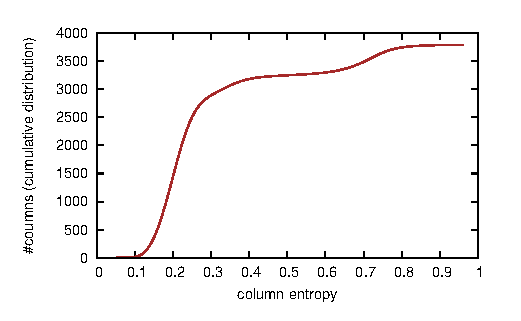
\includegraphics{figs/static/cumul}
\caption{Cumulative distribution of the columns' entropy $\mathcal{E}$.}
\label{fig:cumentr}
\end{figure}

\begin{figure*}[t]
\centering
\tabcolsep2pt
\begin{tabular}{cccc}
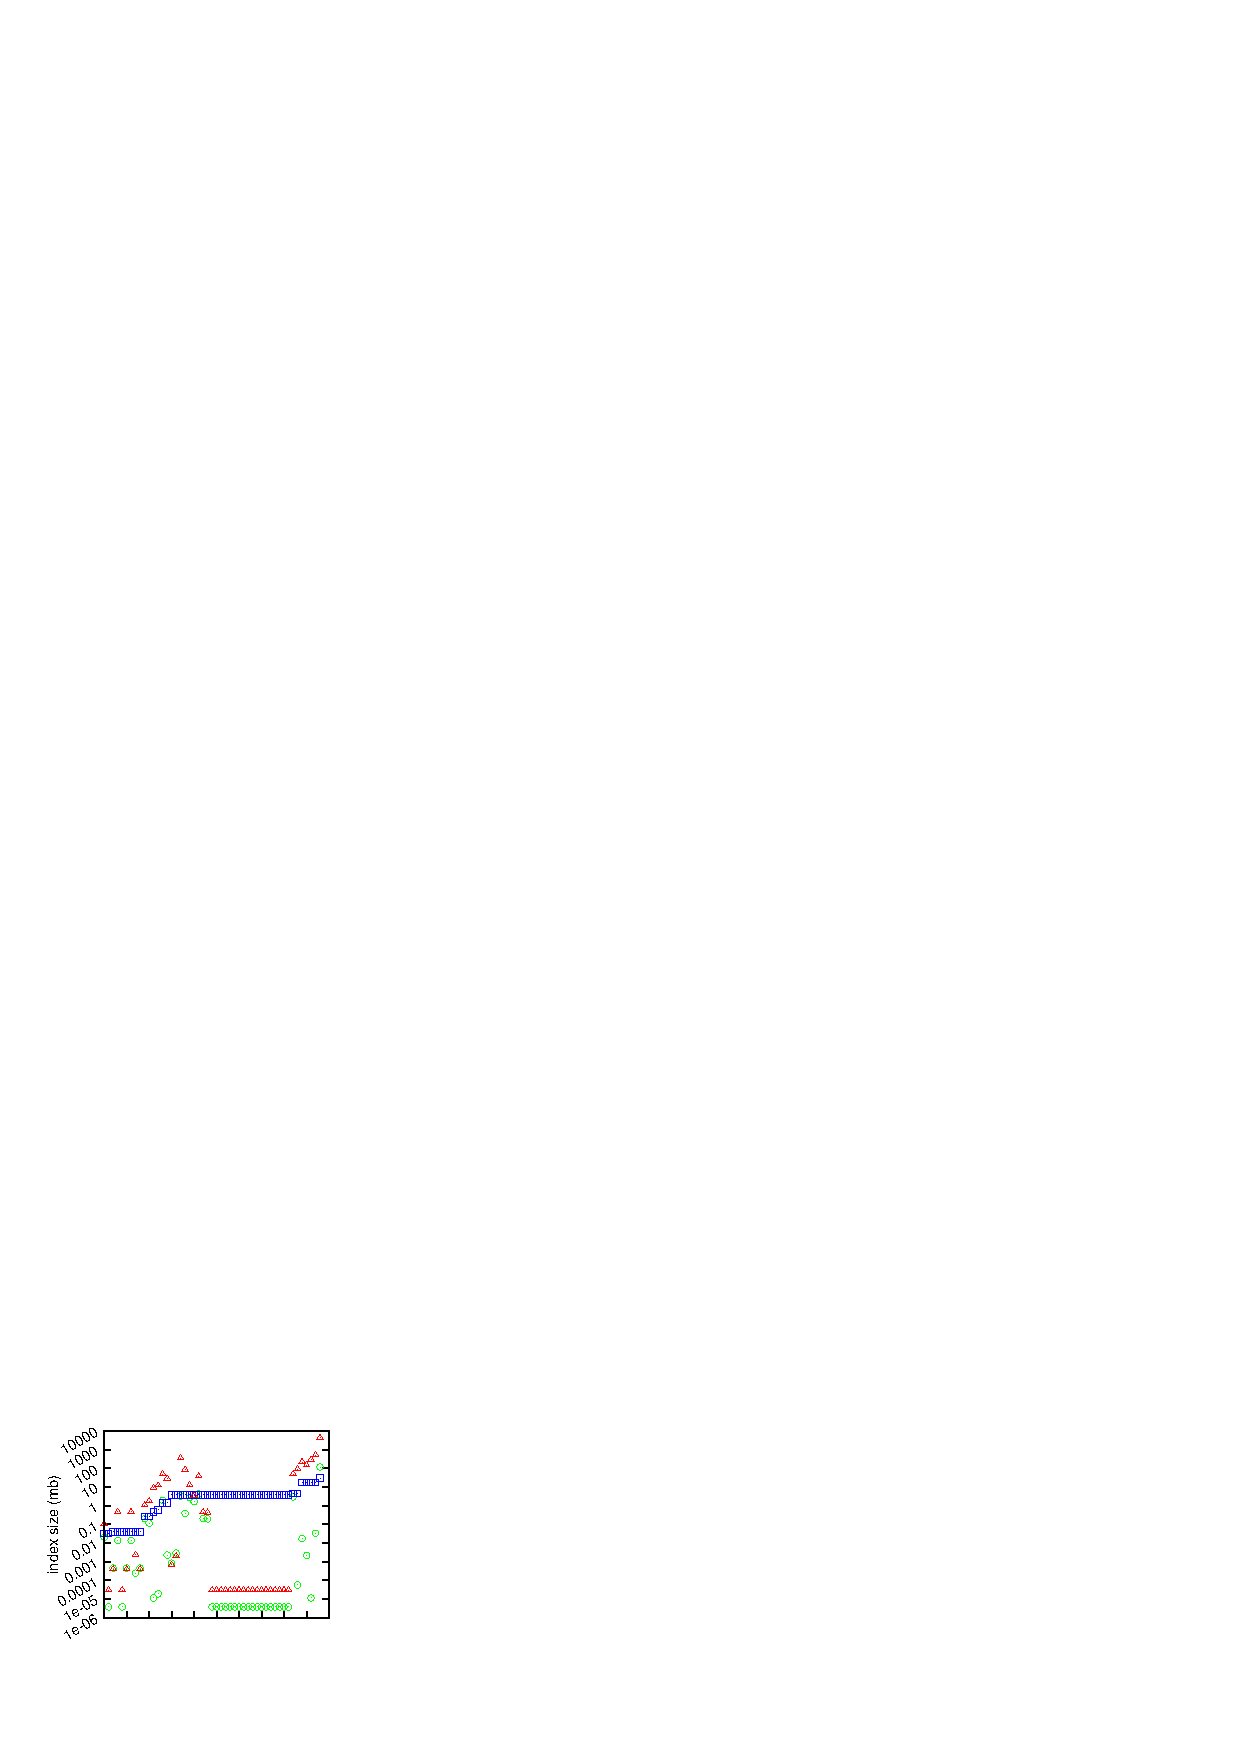
\includegraphics{figs/static/storage_rpp64}&
\includegraphics{figs/static/storage_rpp32}&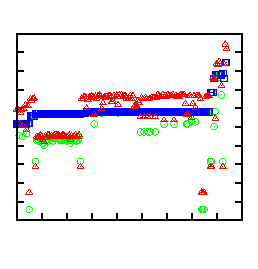
\includegraphics{figs/static/storage_rpp16}&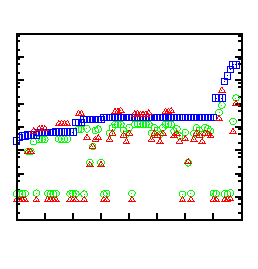
\includegraphics{figs/static/storage_rpp8}\vspace{-15pt}\\
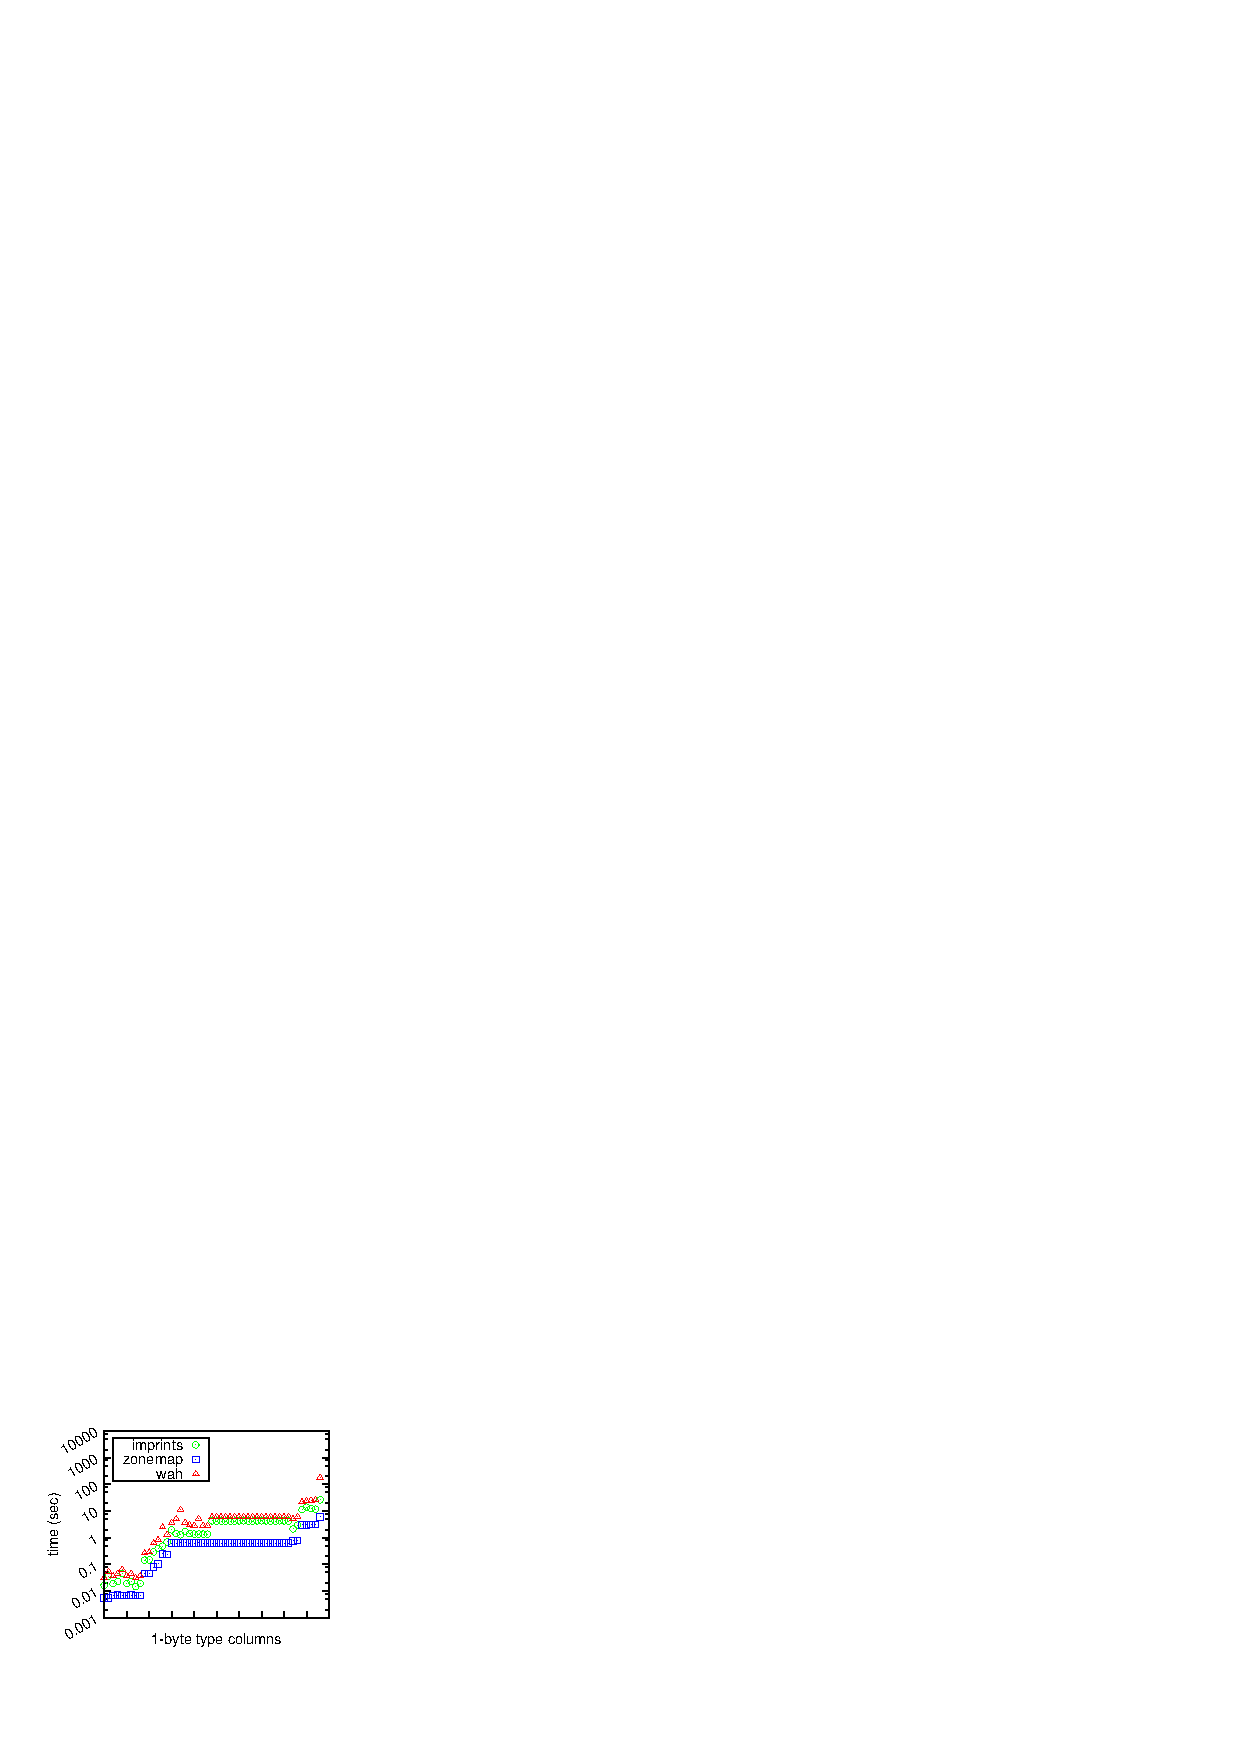
\includegraphics{figs/static/storagetime_rpp64}&
\includegraphics{figs/static/storagetime_rpp32}&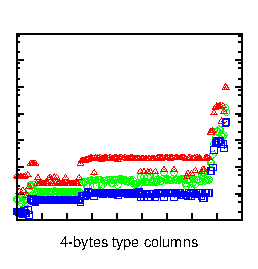
\includegraphics{figs/static/storagetime_rpp16}&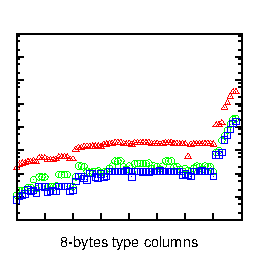
\includegraphics{figs/static/storagetime_rpp8}
\end{tabular}
\caption{Index size and creation time for different types of columns ($x$-axis enumerates the columns, ordered by size).}
\label{fig:storage}
\end{figure*}

Table~\ref{tbl:dataset} lists the name, the size in gigabytes, the total number
of columns, the column types, and the maximum number of rows of the datasets
used for our experimentation. The first dataset, denoted as Routing, is a
collection of over 240 million geographical records (i.e., longitude, latitude,
trip-id, and timestamp) of ``trips'' as logged by gps devices. The next
dataset, SDSS, is a 6.2 GB sample of the astronomy database
SkyServer. This database contains
scientific data, with many double precision and floating point columns
following a uniform distribution, thus stressing compression techniques to their
limits. Cnet is a categorical dataset describing the properties of technological
products. All data are stored on a single but very wide table, where each
column is very sparse, thus presenting ample opportunities for
compression. The dataset was re-created based on the study of
J.Beckham~\cite{cnet}. The Airtraffic delay database represents an ever growing data warehouse with statistics about flight
delays, landing times, and other flight statistics. The data are updated per
month, leading to many time-ordered clustered sequences. Lastly, we used the
TPC-H benchmark dataset with scale factor 100, in order to
compare against a well recognizable dataset.

\subsection{Column Entropy}

We wish to better study the properties of the columns that are typically not
ordered, part of very wide tables, and eligible for secondary indexing. Our
initial motivation was based on the observation that ``secondary data'' exhibit
some degree of clustering, either inherited during the creation process of the
data, or indirectly imposed by the few columns that are ordered because of
primary indexing. Column imprints are designed such that this clustering is
naturally exploited without the need of explicit configuration. This is why
imprints are built per block and compressed row-wise per imprint vector,
instead of vertically per bin.
To better understand and quantify the degree of clustering found in data, we
define a new metric, called \it{column entropy}. Column entropy measures how close
a column is to being ordered, or, in other words, the amount of clustering found
in a column when the values are partitioned into bins. More formally, column
entropy $\mathcal{E}$ is defined to be
$$\mathcal{E}=\frac{\sum^{n}_{i=2}d(i,i-1)}{2\times\sum^{n}_{i=1}b(i)}$$
where $d(i,i-1)$ is the \it{edit distance} between bit-vector $i$ and $i-1$,
and $b(i)$ is the number of bits that are set in bit-vector $i$. We define the
edit distance between two bit-vectors to be the number of bits that need to be
set and unset in the first bit-vector in order to become the second. Column
entropy $\mathcal{E}$ takes values between $0.0$ and $1.0$. The higher the
entropy $\mathcal{E}$ the more random the data is and the less clustered it
appears to be.

To give a more intuitive view of \it{column entropy}, we print a
small portion of the column imprint index of five columns, one from each
dataset, and list them in Figure~\ref{fig:snap}, together with their respective
entropy value $\mathcal{E}$. The prints in Figure~\ref{fig:snap} correspond to
the actual imprint indexes as constructed in our code for the experiments. If a
bit is set then an \tt{`x'} is printed, otherwise an \tt{`.'}. The first
column imprint of Figure~\ref{fig:snap} corresponds to a column from the
SkyServer dataset. It is of type real and has a high entropy value of almost
$0.8$ which implies that each next imprint vector is significantly different
from the previous one. Such columns with high entropy, as demonstrated in the
next section, are harder to compress. The next imprint is the latitude
attribute of the Routing dataset. It exhibits nice clustering properties,
something to be expected since the dataset is taken from real observations, and
thus trips are continuous without any jumps, unless the trip-id changes. The
next two imprints are taken from the Airtraffic and Cnet dataset. These are
categorical datasets, with low cardinality -- hence the smaller bit-vectors --
and with low entropy value. The last imprint index is the \it{retail\_price}
attribute of table \it{part} of TPC-H. This dataset is created to contain a
sequence of prices that are not ordered, but they are still the same repeated
permutation of an order. Such an organization of data resembles closely an
ordered column, and thus also has a low entropy value.

Figure~\ref{fig:cumentr} depicts the cumulative distribution of the entropy
$\mathcal{E}$ for all columns of all datasets that we used in our experiments.
We exclude all columns that are less than $1$ megabyte in size, since
they are of minimal interest and introduce outliers in our measurements. More
than $3000$ columns have entropy smaller than $0.4$, thus supporting our claim
that data often tend to exhibit good local clustering and ordering properties.
Nevertheless, there are almost a thousand columns that have high entropy
values, up to almost $1.0$. Those columns are not to be ignored since they sum
up to over $20$\% of the total data. A secondary index should be immune to such
high entropy, and still be able to take advantage of any opportunities for
compression. In the next section we study the storage overhead of imprints and
other state-of-the-art secondary indexes, while giving emphasis to their
behavior on columns with high entropy. We show that imprints are robust
against columns with high entropy, while bitmaps with WAH fail to achieve a
good compression rate.

\subsection{Index Size and Creation Time}

We analyze the storage overhead introduced by the column imprints index
and compare it with that of zonemaps and WAH. The upper row of the graphs in
Figure~\ref{fig:storage} depict the sizes of the indexes over all columns and
all datasets. Each graph corresponds to a different value type. For
presentation reasons, we divide the types according to their size in bytes. For
example, char is $1$-byte, short is $2$-byte, int and date are
$4$-byte, and long and double $8$-byte types. The $y$-axis depicts the size of
the indexes measured in megabytes, starting from a few bytes for the smaller
columns to almost one gigabyte for the large ones. Notice that $y$-axis is
\it{log-scaled}. The $x$-axis orders the columns according to their size (in
increasing order). However, because many columns have exactly the same size,
since they originate from the same tables, we distinguish them by placing them
next to each other. As a result, the flat horizontal patterns appearing in the
graphs correspond to different columns of the same size, while the
``stepping'' effect corresponds to the next group of larger columns.

\begin{figure}
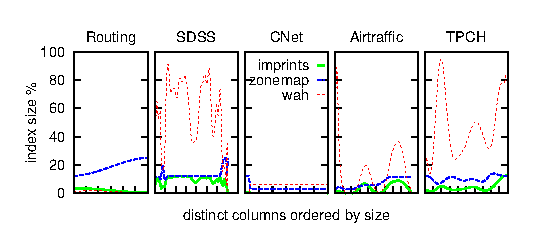
\includegraphics{figs/static/percentage}
\caption{Index size overhead \% over the size of the columns.}
\label{fig:perc}
\end{figure}

The red triangle points mark the size of the bit-binning index with WAH
compression, the blue squares mark the size of zone\-maps, and the green
circles mark the size of the column imprints index. The general
picture drawn for all types is that WAH index entails the largest storage
overhead, zonemaps come second, while imprints have the least
requirements of storage space. More specifically, the general trend is that
imprints are between one and two orders of magnitude more space efficient
than zonemaps and WAH. However, there are exceptions to that rule, especially
for WAH indexing, which depicts the biggest fluctuation in storage needs. For
$1$-byte types, there are cases where WAH achieves better compression and
reaches that of imprints. By examining the data closer we noticed that this is
true for columns that although they have more than 126 million rows (taken from
the Airtraffic dataset), they only contain two distinct values, thus allowing
both WAH and imprints to fully compress their bit-vectors. Another point of
interest is found in the case of $8$-byte types, where WAH can become a bit
more space efficient than imprints. This is true for those columns that contain
primary keys (e.g., bigint identifiers) and in addition are ordered.
Although we are studying secondary indexes that typically apply to unordered
columns, we did not exclude any ordered columns from our experimental datasets
for completeness.

Since it is impractical and hard to explicitly show the size of each individual
column, we compute the percentage of the size of the indexes over the size of
the column. Figure~\ref{fig:perc} shows such a graph. In addition, instead of
grouping on value type, we group columns from the same datasets together, such
that more insights about the different applications, and hence different value
distributions can be gained. The categorical data Cnet which has columns with
low cardinality, as well as the nicely clustered routing dataset, achieve the
best compression for both imprints and WAH, thus requiring in many cases
less than 10\% space overhead. However, the same can not be said for broader
value domains and uniform distributions. Specifically, the scientific
dataset of SkyServer, consisting of many columns with real and double values,
with high cardinality and no apparent clustering, makes the WAH index very
unstable and induces high storage overhead. Imprints perform fairly stably
and much better than WAH, with space overhead closer to zonemaps. The failure
of WAH is expected due to the high randomness of the values in SkyServer, which
allows for very few compression opportunities. However, imprints do not suffer
from the same problem. Since one imprint vector is constructed for each
cacheline, the space requirements are less than bitmaps, while the chance of
consecutive imprint vectors to be identical, and thus compressible, is
increased.

Figure~\ref{fig:entropy} depicts the index size overhead of both imprints
and WAH as percentage of the size of the column, ordered over the entropia
$\mathcal{E}$. Imprints achieve storage overhead less than 10\% for
columns with low entropy, i.e., up to $0.4$. The same observation holds with
few exceptions for WAH indexing. However, the picture changes for columns with
entropy of $0.5$ and higher. Imprints exhibit a steady storage overhead
that hardly exceeds 12\%. WAH indexing suffers more, with up to almost 100\% of
storage overhead on the size of the column. Imprints on the one hand need
at most 64 bits per cacheline unit, making them immune to high entropy,
while benefiting from low entropy. On the other hand, WAH can potentially
become very inefficient. If there are very few opportunities for compression,
most 32-bit words will be aligned with 31-bit literals, i.e., no big long
sequences of same bits will be found in the bit-vectors. In addition, since we
use a 64 bit-binning approach, there will potentially be 64 uncompressed bits
per value. All in all, WAH is more suitable for low entropy data, while
imprints are more stable and with better compression for the entire range of
entropy values, i.e., they work even if data are not locally clustered.

\begin{figure}
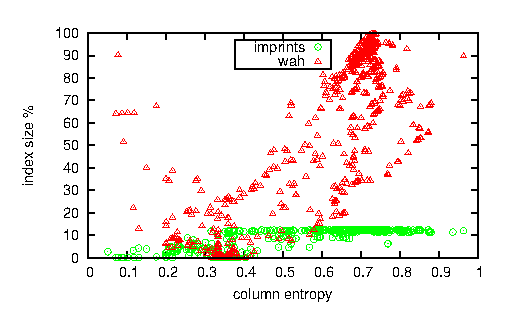
\includegraphics{figs/static/entropy}
\caption{Index size overhead \% over column entropy $\mathcal{E}$.}
\label{fig:entropy}
\end{figure}

Another concern is the time spent to create each secondary index. The bottom
row of graphs in Figure~\ref{fig:storage} depicts the creation time for WAH,
zonemaps, and imprints. As expected the zonemaps are the fastest to create.
For each row only two comparisons have to be made to determine the minimum
and the maximum values for the current zone. The slowest is the WAH index,
since there is significantly more work to be done in order to compress the
bit-vectors. Imprints on the other hand, always perform between zonemaps and
WAH. The overall differences of the construction time between the three indexes
is steady and to be expected since each of them require a different amount of
work per value. Most importantly, the time for all indexes increases linearly
to the size of the columns, thus making them a cost-effective solution for
secondary indexing.

\subsection{Query Performance}

Next, we turn our attention to the performance analysis of evaluating range
queries. The execution scenario for this set of experiments is as follows. For
each column, ten different range queries with varying selectivity are created.
The selectivity starts from less than $0.1$ and increases each time by
$0.1$, until it surpasses $0.9$. These 10 queries are then fired against the
three indexes (i.e., zonemaps, WAH, and imprints) defined over the column,
and also evaluated with a complete scan over that column. The result set of
each query is a materialized ordered list of \it{id}'s. The ordering of
\it{id}'s is guaranteed by the sequential scan, the zonemap index, and the
imprints index. However, this is not true for WAH, since each pass over the
different bit-vectors will produce a new set of \it{id}'s which needs to be
merged. The merging is done by defining another bit-vector aligned with the
\it{id}'s. The bits that are set in this \it{id} bit-vector correspond to the
\it{id}'s that satisfy the range query. In this way no final merge is needed,
just the materialization of the \it{id}'s. This implementation only adds a
small, but necessary for fairness, overhead to WAH compared to the other
indexes.

\begin{figure}
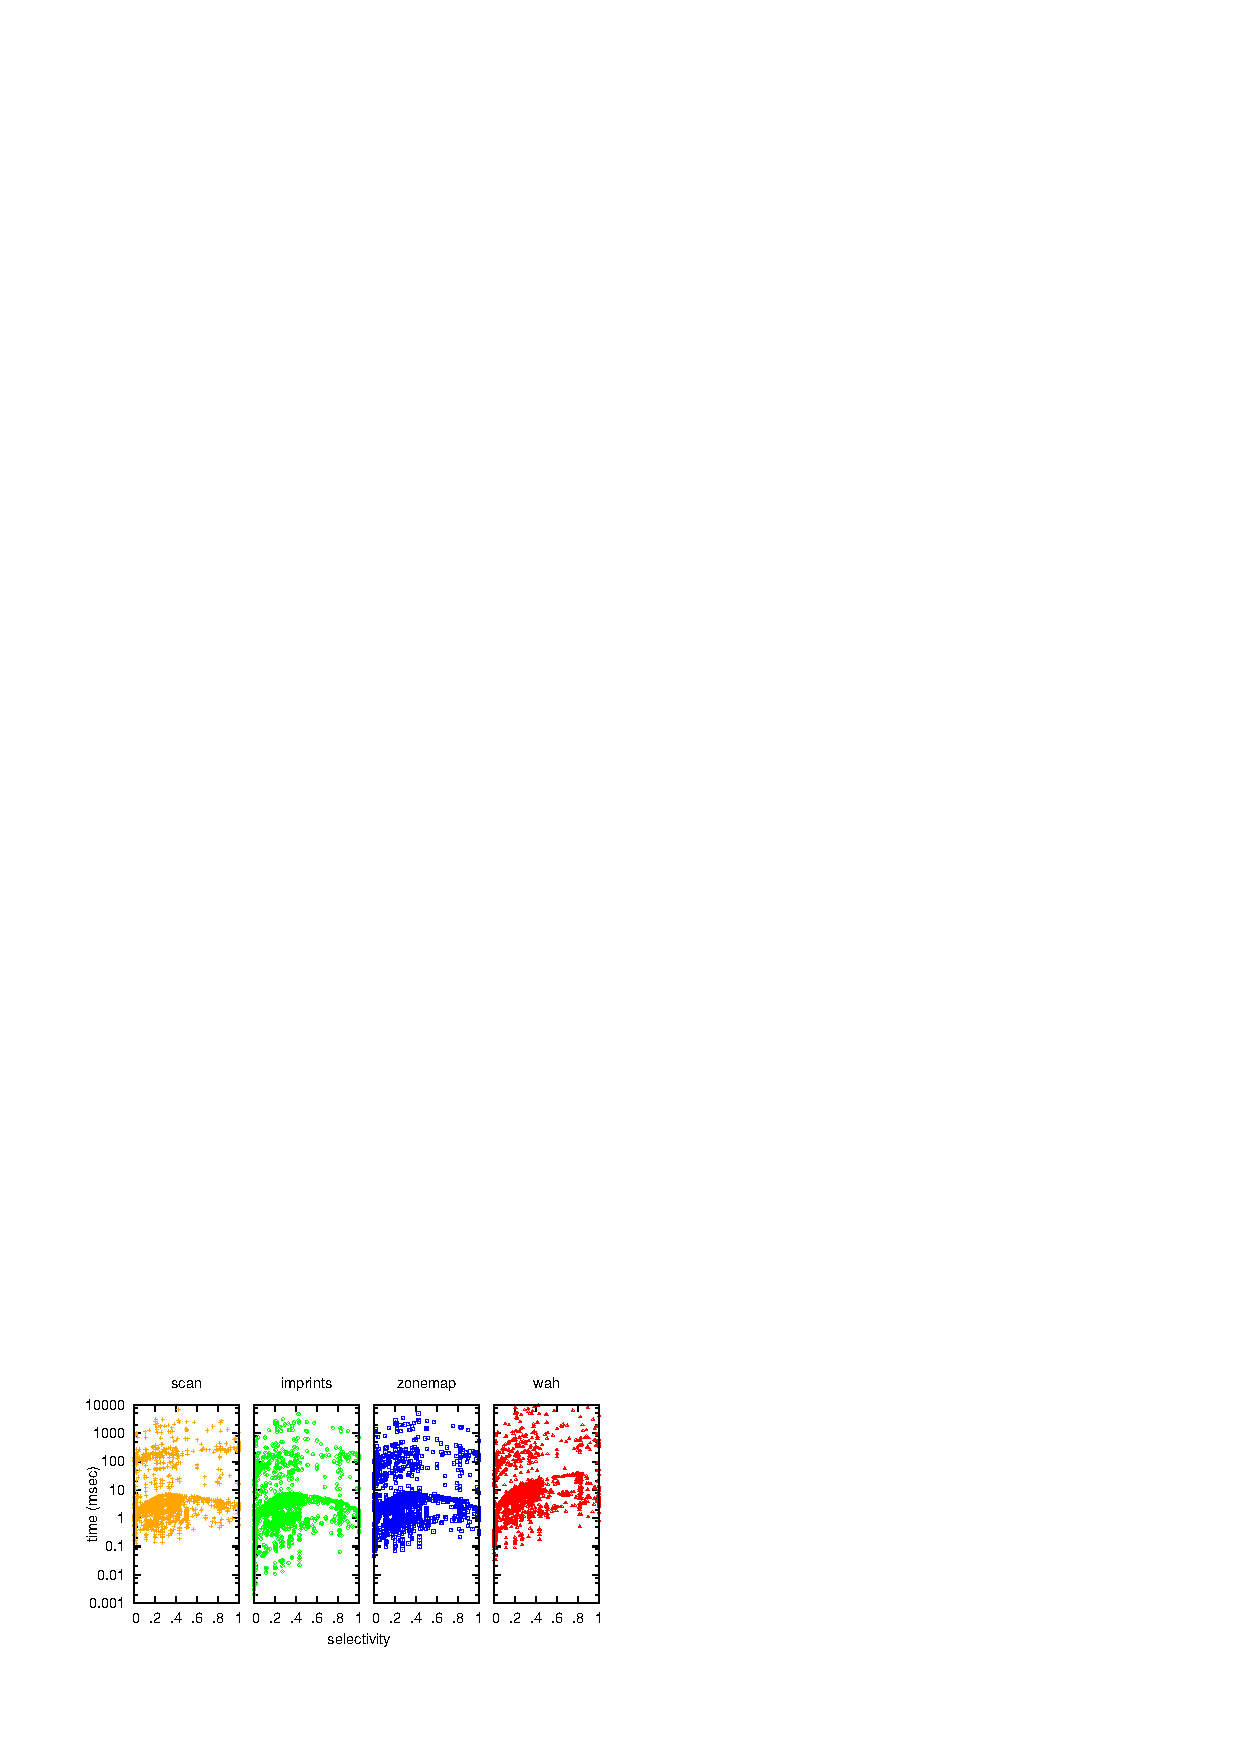
\includegraphics{figs/static/qtime}
\caption{Query time for decreasing selectivity.}
\label{fig:queryt}
\end{figure}

Figure~\ref{fig:queryt} plots the query times of over 40,000 queries evaluated
over each index. The queries are ordered on the $x$-axis according to their
selectivity. If the selectivity is $0.1$, the query returns 10\%
of the total values in the column, while $0.9$ returns 90\% of the total
values. All three indexes and the sequential scan produce the same graph
patterns for query times. However, these patterns are shifted along the
$y$-axis. Imprints is the fastest index overall since the points in the graph
are shifted the most to the bottom. As expected, if the selectivity of the
query is low and thus more data are returned, the smaller the differences that
are observed between indexes. In fact, sequential scans then also become
competitive. This is due to the fact that the overhead of decompressing
the data, and materializing almost all of the \it{id}'s,
surpasses the time needed to sequentially scan the entire column and check each
value. In addition, zonemaps exhibits query times similar to that of
sequential scan for low selectivity queries, since zonemaps require the least
administration overhead compared to imprints and bitmaps with WAH.

\begin{figure}
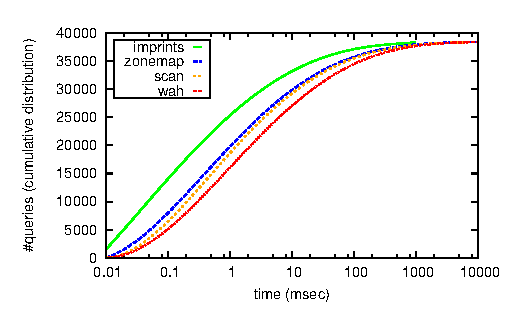
\includegraphics{figs/static/cum_queries}
\caption{Cumulative distribution of query times.}
\label{fig:queryc}
\end{figure}

To better understand the behavior of zonemap, WAH, and imprints, for
queries with high selectivity, and compare them with sequential scans, we
plot in Figure~\ref{fig:queryc} the cumulative distribution of the queries over
time. More precisely, we count the queries that finish execution at each time
frame, and cumulatively sum them up. The steeper the graph in
Figure~\ref{fig:queryc} the more queries finish in a shorter time, thus the
more efficient the index is overall. Figure~\ref{fig:queryc} shows that almost
$15,000$ queries need each of them less than $0.1$ milliseconds to be evaluated
with imprints index. Zonemaps, which is the second best, manage to evaluate
just over 7,500 queries in the same time frame. However, as the evaluation
time increases the time gap between the different approaches is reduced.

\begin{figure}
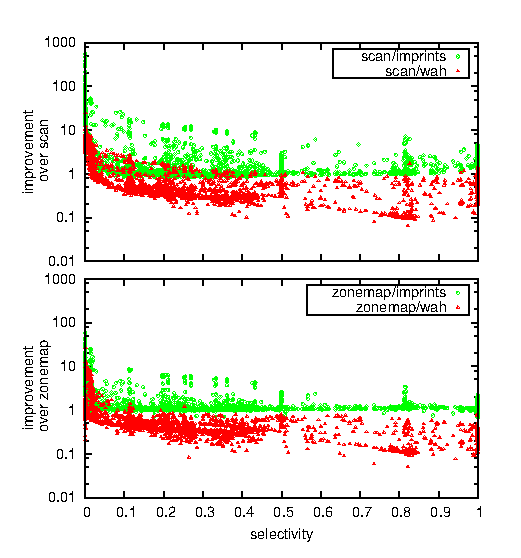
\includegraphics{figs/static/improv}
\caption{Factor of improvement over scan and zonemap.}
\label{fig:impr}
\end{figure}

We are interested in the factor of improvement that is achieved by
the imprints index over the sequential scan baseline and the competitive
zonemap indexing. Figure~\ref{fig:impr} depicts the factor of improvement
achieved for each query. A point above $1$ is translated as a factor of
improvement over the baseline, while a point below $1$ shows how many times
an approach is slower than the baseline. The upper graph of
Figure~\ref{fig:impr} shows with green circle points the improvement of
imprints over sequential scans, while the red triangles, the corresponding
improvement of bitmaps with WAH over sequential scans. Both imprints and WAH,
show a significant improvement for queries with high selectivity, i.e., when
less than 20\% of the tuples are returned. For imprints that improvement is in
some cases almost a $1000$ times faster, and for WAH over $10$. However, for
low selectivity queries, imprints become less competitive, while WAH can become
significantly slower than scans. This observation is aligned with the strategy
of most modern database systems, where, if the cost model of the query
optimizer detects a low selectivity selection, a sequential scan is preferred
over any index probing. Moreover, WAH is punished in a main memory setting. The
processing overhead of the WAH compression outweighs the throughput of data
that is achieved from main memory to the cpu cache. Therefore, WAH is more
suitable for cases where data do not reside in memory, but need to be fetched
from disk. Similarly, the bottom graph of Figure~\ref{fig:impr} depicts the
same comparison, but with zonemap indexing being the baseline, instead of
sequential scans. The same trend can be seen here, although zonemaps is more
competitive and thus the improvement factor for imprints is closer to $100$
times. However, in a few cases of low selectivity zonemaps can become faster
than imprints due to less computation needs.

\begin{figure}
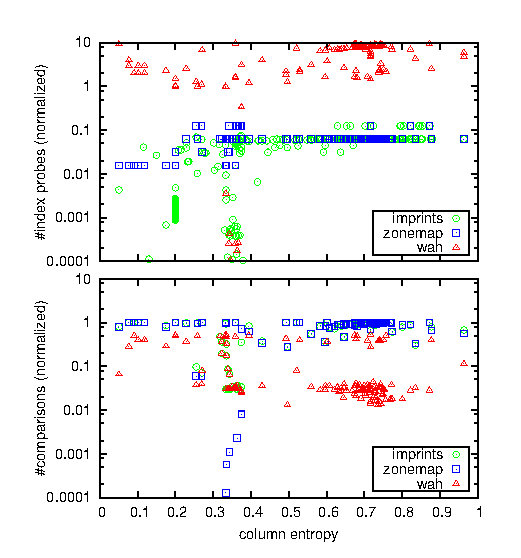
\includegraphics{figs/static/stats}
\caption{Number of index probes and value comparisons for queries with selectivity between $0.4$ and $0.5$.}
\label{fig:stats}
\end{figure}

Finally, we compare the number of index probes and data comparisons performed (originating from testing for false positives) normalized over the number of
records in a column. This experiment reveals implementation-independent
statistics for column imprints in comparison with zonemaps and WAH. The top
graph of Figure~\ref{fig:stats} shows the number of index probes, while the
bottom the number of comparisons, for all queries with selectivity between
$0.4$ and $0.5$. The number of index probes for WAH is the highest of all
indexes, almost always more than the number of total records. This is true
since for each record many bit vectors have to be probed. However, WAH achieves
the best filtering since the number of data comparisons is usually very low. On
the other hand, zonemaps have a steady number of index probes, i.e., exactly
the number of cachelines of the column. The number of comparisons for zonemaps
depends on the data skew and can vary. Column imprints achieve a balance
between index probes and data comparisons. Columns with high entropy entail
more index probes but less data comparisons. On the
other hand, columns with low entropy will need less index probes but more data
comparisons.

In conclusion, for high selectivity queries column imprints index can achieve a
factor of $1000$ improvement over sequential scans, and a factor of $100$ over
zonemap. Further experimentation, revealed that there is a correlation between
the query evaluation time and the sizes of the column, or the size of the
index, which in turn is correlated with the column entropy. We do not show
these graphs since they do not reveal any new insights into the performance of
imprints compared to zonemap or WAH index.

\section{Conclusions and Future Work}\label{sec:conclusions}

Column imprints is a light-weight secondary index with a small memory
footprint suited for a main-memory setting. It belongs to the class of
bitvector indexes, which has a proven track record of improving access in
large-scale data warehouses. Our extensive experimental evaluation
shows significant query evaluation speed-up against pure scans and the
established indexing approaches of zonemaps and bitmaps with bit-binning and
WAH compression. The storage overhead of column imprints is just a few percent,
with a max of 12\% over the base column.

Column imprints can be extended to exploit multi-core
platforms during the construction phase and during multi-attribute query
processing. Akin to prevailing techniques, such as~\cite{SW07,WMC10}, judicious
choice of the binning scheme, and a multi-level imprints organization, may
lead to further improvements in specific application domains.

\bibliographystyle{abbrv}
{\small\bibliography{bibliography}}
%\bibliography{bibliography}
\end{document}
